\documentclass{classes/memoire}
\usepackage{minted}
\setminted[]{
    xleftmargin=.75cm,
    xrightmargin=.75cm,
    frame=single,
    framesep=.25cm,
    linenos,
    tabsize=2,
    breaklines
}
\usepackage{listings}
% \lstset{language=YAML}
\lstdefinestyle{yaml}{
     basicstyle=\color{blue}\footnotesize,
     rulecolor=\color{black},
     string=[s]{'}{'},
     stringstyle=\color{blue},
     comment=[l]{:},
     commentstyle=\color{black},
     morecomment=[l]{-}
 }

\usepackage{lmodern}
\usepackage{garamond}
\usepackage{comment}
\usepackage{geometry}
\usepackage[options]{nohyperref}
% \PassOptionsToPackage{russian}{babel}
 % \geometry{
 % a4paper,
 % total={170mm,257mm},
 % left=20mm,
 % top=20mm,
 % }
\renewcommand\lstlistoflistingscaption{List of source codes}
\renewcommand{\mtctitle}{Table of contents}
\begin{document}
%\frontmatter

%----------------------------------------------------------------------------------------
%	TITLE PAGE
%----------------------------------------------------------------------------------------

\thispagestyle{empty}
 \begin{tikzpicture}[remember picture,overlay]
   \node at (current page.center) {
\includegraphics[width=\pdfpagewidth,height=\pdfpageheight]{frontmatter/remerciements/Page-de-garde-YoussefMarzouk-03.png}};
 \end{tikzpicture}
\clearpage



%----------------------------------------------------------------------------------------


%----------------------------------------------------------------------------------------
%	TITLE PAGE
%----------------------------------------------------------------------------------------

\thispagestyle{empty}
 \begin{tikzpicture}[remember picture,overlay]
   \node at (current page.center) {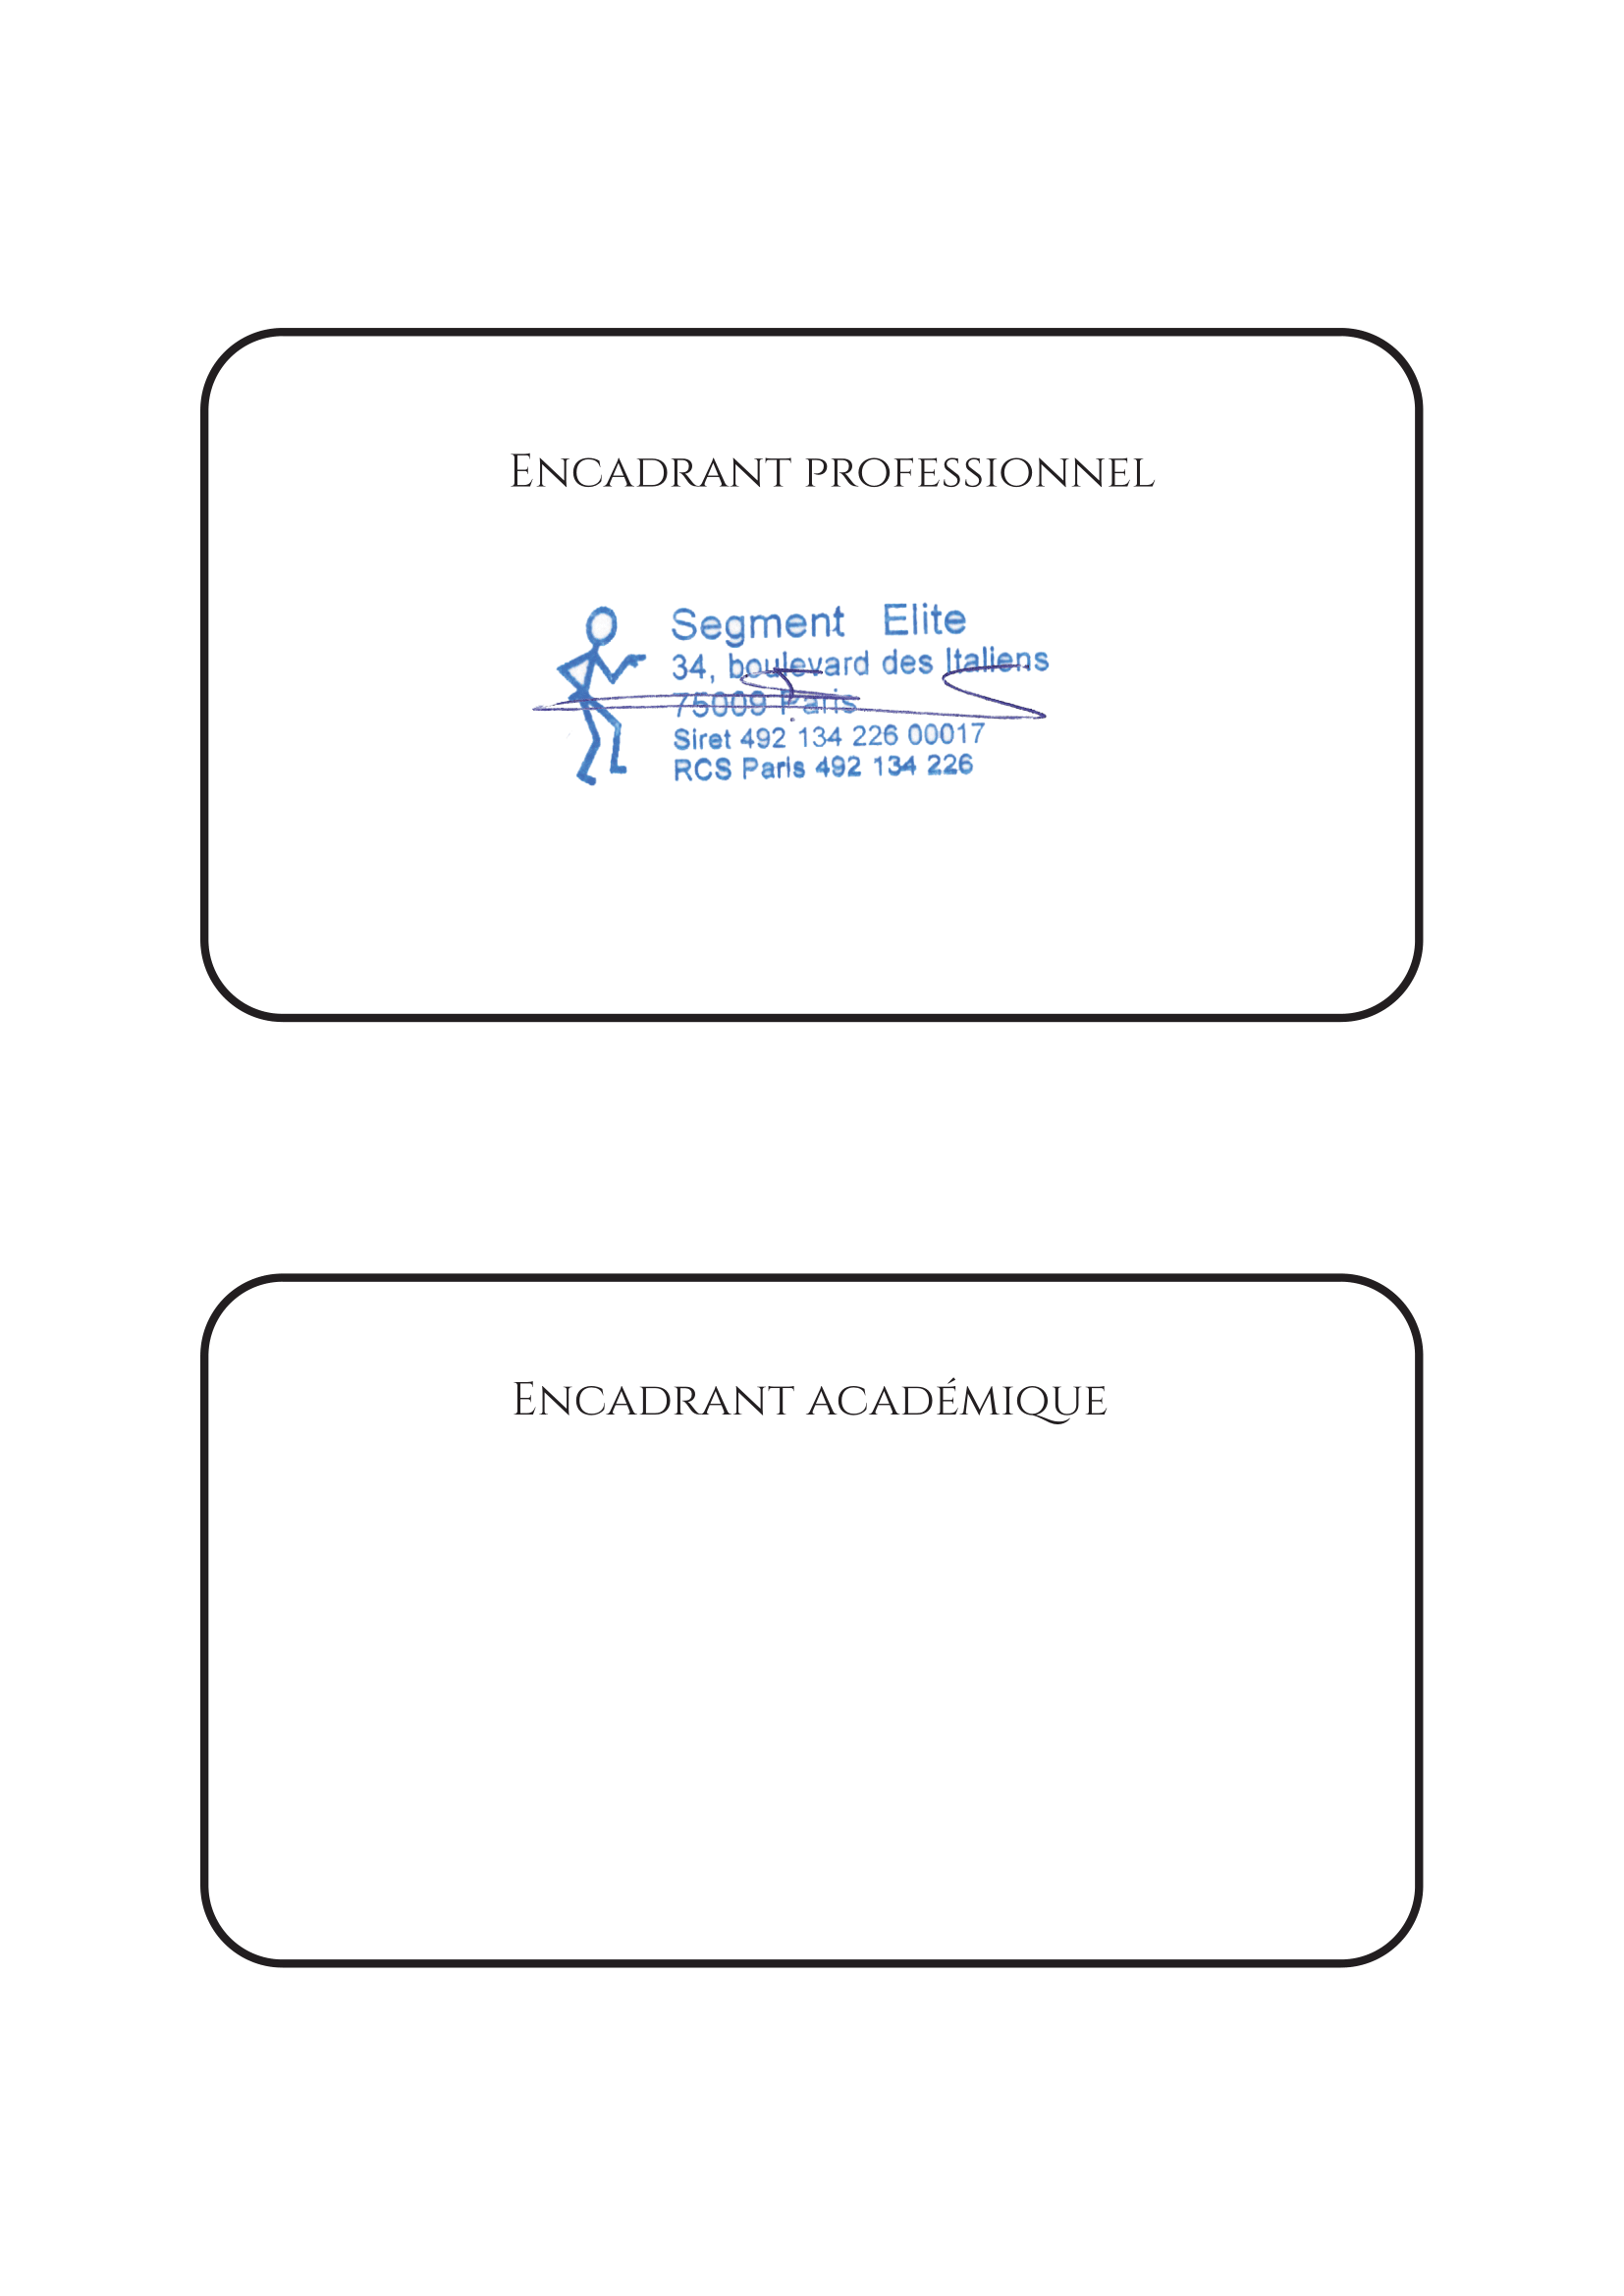
\includegraphics[width=\pdfpagewidth,height=\pdfpageheight]{frontmatter/signature/signed-v1.png}};
 \end{tikzpicture}
\clearpage



%----------------------------------------------------------------------------------------

%\garamond
\thispagestyle{empty}
\thispagestyle{empty}
\begin{center}
\ungaramond{\textbf{\LARGE{Resumé}}}
\end{center}
\vspace{0.8cm}

Le\textcolor{white}{J}présent\textcolor{white}{J}travail\textcolor{white}{J}est\textcolor{white}{J}fait\textcolor{white}{J}dans\textcolor{white}{J}le\textcolor{white}{J}cadre\textcolor{white}{J}d’un\textcolor{white}{J}projet\textcolor{white}{J}de\textcolor{white}{J}fin\textcolor{white}{J}d’études\textcolor{white}{J}pour\textcolor{white}{J}obtenir\textcolor{white}{J}le\textcolor{white}{J}
diplôme\textcolor{white}{J}national\textcolor{white}{J}d’ingénieur\textcolor{white}{J}en\textcolor{white}{J}informatique\textcolor{white}{J}à\textcolor{white}{J}l’école\textcolor{white}{J}supérieure\textcolor{white}{J}privée\textcolor{white}{J}et\textcolor{white}{J}de\textcolor{white}{J}
technologie\textcolor{white}{J}ESPRIT. Le stage est fait chez L'oreal. Ce projet de fin d’étude consiste à concevoir et développer une plateforme intitulé "Fast alignement" permettant un alignement entre le chimiste et le marketeur en matière de choix et de validation des teintes de couleur de cheveux à mettre en production.

Mots clés : .NET Core,ReactJS,Cosmos DB,Ray Tracing.

\\
\vspace{2cm}
\begin{center}
\ungaramond{\textbf{\LARGE{Absract}}}
\end{center}
\vspace{0.8cm}
The\textcolor{white}{J}present\textcolor{white}{J}work\textcolor{white}{J}is\textcolor{white}{J}done\textcolor{white}{J}as\textcolor{white}{J}part\textcolor{white}{J}of\textcolor{white}{J}an\textcolor{white}{J}end-of-studies\textcolor{white}{J}project\textcolor{white}{J}to\textcolor{white}{J}obtain\textcolor{white}{J}the\textcolor{white}{J}national\textcolor{white}{J}
diploma\textcolor{white}{J}of\textcolor{white}{J}computer\textcolor{white}{J}engineer\textcolor{white}{J}at\textcolor{white}{J}the\textcolor{white}{J}private\textcolor{white}{J}higher\textcolor{white}{J}school\textcolor{white}{J}and\textcolor{white}{J}technology 
ESPRIT.
The internship is done at L'Oreal. This end-of-study project consists of designing and developing a platform entitled "Fast Alignment" allowing alignment between the chemist and the marketer in terms of the choice and validation of the hair color shades to be put into production.

Keywords .NET Core,ReactJS,CosmosDB,Ray Tracing

\begin{flushright}
\textbf MARZOUK Youssef
\end{flushright}
\thispagestyle{empty}
\thispagestyle{empty}
\begin{center}
\ungaramond{\textbf{\LARGE{Dedications}}}
\end{center}
\vspace{0.8cm}

I would like to dedicate this end-of-studies project to all the people who supported me throughout my professional and personal career. I am grateful to the following individuals: 

My parents for their unwavering love and support throughout my life. I owe them for everything they have done for me, and I am grateful to have them as family. 

My brother, Mr. Rafick Bouazizi, who sponsored my education, for his financial and moral support throughout my academic journey. Without his help, I would not have been able to achieve my educational goals. 

All my family members for their unconditional love and support throughout my life. I am grateful to have them as family and I am grateful for their support and encouragement. 

My friends for their support, friendship, and encouragement throughout my academic and professional journey. Their support and presence helped me through the ups and downs of life and to persevere in my efforts. 

I am grateful to all these people for their support and encouragement, and I dedicate this project to them with gratitude and appreciation.
\begin{flushright}
\textbf Ridha Bouazizi
\end{flushright}

\newpage
\thispagestyle{empty}
\begin{center}
\ungaramond{\textbf{\LARGE{Dédicaces}}}
\end{center}
\vspace{0.8cm}

Je voudrais dédier ce travail de fin d'études à toutes les personnes qui m'ont soutenu tout au long de mon parcours professionnel et personnel. Je suis reconnaissant envers les personnes suivantes : 

Mes parents pour leur amour et leur soutien indéfectibles tout au long de ma vie. Je leur suis redevable pour tout ce qu'ils ont fait pour moi et je suis reconnaissant de leur avoir comme famille. 

Mon frère, M. Rafick Bouazizi, qui a sponsorisé mon éducation, pour son soutien financier et moral tout au long de mon parcours universitaire. Sans son aide, je n'aurais pas pu atteindre mes objectifs éducatifs. 

Tous les membres de ma famille pour leur amour et leur soutien inconditionnels tout au long de ma vie. Je suis reconnaissant de les avoir comme famille et je leur suis reconnaissant pour leur soutien et leur encouragement. 

Mes amis pour leur soutien, leur amitié et leur encouragement tout au long de mon parcours universitaire et professionnel. Leur soutien et leur présence m'ont aidé à traverser les hauts et les bas de la vie et à persévérer dans mes efforts. 

Je suis reconnaissant envers toutes ces personnes pour leur soutien et leur encouragement, et je leur dédie ce travail avec gratitude et reconnaissance.

\begin{flushright}
\textbf Ridha BOUAZIZI
\end{flushright}
%\justify
\pagenumbering{Roman}
\begin{center}
\ungaramond{\textbf{\LARGE{Remerciements}}}
\end{center}
\vspace{0.8cm}        % ne pas numéroter

C’est avec un grand plaisir que je réserve cette page en signe de gratitude envers toutes les
personnes ayant participé de près ou de loin dans l’élaboration de ce travail.
\\
Mes premiers remerciements vont à : Mon encadrant M. TROUDI Azer, pour son accueil, sa disponibilité et la qualité de l’encadrement dont il m’a fait bénécier tout au long de ce stage.
Je remercie, également, tout les membres de l'equipe pour leur collaboration et l’expérience professionnelle acquise.
\\
Je tiens à présenter mes reconnaissances et mes remerciements à mon Superviseur à ESPRIT Mme. REJEB Nejla qui a bien voulu assurer la direction de ce travail. Je le remercie infiniment pour sa patience, son assistance et ses précieuses recommandations.
%\ungaramond
%\pagestyle{empty}
\dominitoc 
\tableofcontents
\listoftables 
\listoffigures

\lstlistoflistings
%\garamond
%% \thispagestyle{empty}
% \begin{center}
% \ungaramond{\textbf{\LARGE{Glossaire}}}
% \end{center}
% \vspace{0.8cm}
% \textbf{PO:} Product Owner
% \newline
% \textbf{BD:} Base de Données
% \newline
% \textbf{UI:} User Interface
% \newline
% \textbf{MS:} Microservices
% \newline
% \textbf{UML:} Le Langage de Modélisation Unifié, de l'anglais Unified Modeling Language
% \newline
% \textbf{PDF:} Portable Document Format
% \newline
% \textbf{IDE:} Un environnement de développement intégré (abrégé EDI en français ou IDE en anglais, pour Integrated Development Environment)
% \newline
% \textbf{JAVA EE:} Java Entreprise Edition
% \newline
% \textbf{AOP:} Programmation Orientée Aspects
% \newline

\pagestyle{fancy}
\fancyhead[L]{\ungaramond\small\textbf{}}
\fancyhead[C]{}
\fancyhead[R]{\ungaramond\small\textbf{}}
\fancyfoot[L]{\ungaramond\small\textbf{Ridha Bouazizi}}
\fancyfoot[C]{}
\fancyfoot[R]{\ungaramond\small\textbf{Page \thepage\ sur\ \pageref{LastPage}}}
\renewcommand{\headrulewidth}{1.7pt}
\renewcommand{\headrule}{\hbox to\headwidth{\color{gray}\leaders\hrule height \headrulewidth\hfill}}
\renewcommand{\footrulewidth}{1.7pt}
\renewcommand{\footrule}{\hbox to\headwidth{\color{gray}\leaders\hrule height \footrulewidth\hfill}}
\pagenumbering{arabic}
\phantomsection\addcontentsline{toc}{chapter}{General topic } % inclure dans TdM
\begin{center}
\ungaramond{\textbf{\LARGE{General topic }}}
\fancyhead[R]{\ungaramond\small\textbf{General topic }}

\end{center}
\vspace{0.8cm}
\setcounter{page}{1}


Our project aims to put in place a complete Platform as a Service (PaaS) environment in the cloud and implement the standard DevOps best practices to improve software delivery and operational efficiency. 

Cloud computing has revolutionized the way we deploy and manage software applications, offering greater flexibility, scalability, and cost savings. 

PaaS is a cloud-based service that provides developers with a platform to build, deploy, and manage applications without the need for infrastructure management. PaaS allows organizations to focus on developing and delivering software applications rather than managing the underlying infrastructure. 

DevOps is a set of practices that emphasizes collaboration and communication between development and operations teams to improve software delivery and operational efficiency. DevOps aims to break down the silos between development, operations, and other IT functions to create a more efficient and effective software delivery pipeline. 

Our project will focus on implementing the Agile DevOps method to improve collaboration between development and operations teams, automate software delivery pipelines, and increase the speed of software delivery. We will use a variety of tools and technologies, including containerization, continuous integration and deployment, and infrastructure automation to achieve our goals. 

We believe that our project will provide a valuable contribution to the field of cloud computing and DevOps by demonstrating how the Agile DevOps method can be used to improve software delivery and operational efficiency in PaaS environments. 

We look forward to sharing our results and findings with the community and contributing to the ongoing evolution of these important fields.

\graphicspath{{./assets/}}
\setcounter{mtc}{1}
\chapter{Generalized context of the project }
\fancyhead[R]{\ungaramond\small\textbf{Chapter I. Generalized context of the project}}
\minitoc
\newpage
\section*{Introduction}
The Generalized context of a project is a crucial aspect that outlines the scope, purpose, and objectives of the project. For an end of study project in the fields of cloud computing and DevSecOps, the Generalized context of the project is critical in providing a comprehensive understanding of the project's goals and expected outcomes. 

Cloud computing is a technology that enables users to access computing resources, such as servers, storage, applications, and services, over the internet on a pay-per-use basis. DevSecOps, on the other hand, is an approach that integrates security into the software development and operations process. 

This chapter provides a comprehensive overview of the project's context, including the problem statement, objectives, and scope. It aims to provide a clear understanding of the project's purpose and the expected outcomes

\section{Overview on the host organization  }

\subsection{Company Background }
Systnaps is a technology company based in Paris, France that specializes in providing innovative software solutions to businesses across various industries. It prides itself with the expertise in areas such as data analytics, artificial intelligence, machine learning, and cloud computing. The following figure illustrates the company logo: 

\begin{figure}[!ht]\centering

\includegraphics[width=0.5\textwidth,angle=00]{assets/fa.png}
\caption{Systnaps Logo}
\end{figure}

Huxium, a subsidiary organization of Systnaps is a technology company that specializes in providing customized software solutions to businesses across various industries. 


\begin{figure}[!ht]\centering

\includegraphics[width=0.5\textwidth,angle=00]{assets/fb.png}
\caption{Huxium Logo}
\end{figure}


 \subsection{Mission and Vision }

Systnaps was founded with the mission of helping businesses harness the power of technology to improve their operations, enhance customer experiences, and drive growth. They offer a range of services to meet the diverse needs of their clients, including custom software development, application maintenance and IT consulting. 

\subsection{Core Services or Products }

The core services of Systnaps in the data management space include: 
\begin{itemize}[label={--}]
    \item Database Management: Systnaps offers services to help businesses manage their databases, ensuring their data is secure and available when needed. This includes tasks such as database administration, performance optimization, and disaster recovery. 

\item Data Integration: Systnaps offers services to help businesses integrate and manage their data across multiple systems and platforms. This includes tasks such as data migration, data warehousing, and data synchronization. 

\item Big Data: Systnaps offers services to help businesses manage and analyze large volumes of data, often referred to as "big data". This includes tasks such as data processing, data visualization, and machine learning. 

\item  Data Governance: Systnaps offers services to help businesses ensure that their data is being managed in compliance with regulatory and legal requirements. This includes tasks such as data privacy and security, data classification, and data retention. 

 \end{itemize}

\subsection{Market Position and notable clients }

While they do not have a significant global presence, they have established themselves as a reputable player in the French IT market. 

Systnaps has worked with clients across a range of industries, including finance, healthcare, and media. The following figure showcases some of the current clients: 


\begin{figure}[!ht]\centering

\includegraphics[width=0.8\textwidth,angle=00]{assets/fc.png}
\caption{Company clients}
\end{figure}


\section{Project description }

Our end of studies project involves designing and implementing, on the cloud, a complete platform as a service (PaaS) solution that incorporates a range of services related to networking, storage, and automation. 

Specifically, this project involves designing and implementing a PaaS platform that includes a range of networking services, such as load balancing, ingress, and authentication/authorization, which are essential for managing traffic flow and ensuring secure access to the platform. 

The project also involves implementing a distributed and redundant storage backend that includes both object and block storage to ensure reliable and scalable storage capabilities. 

In addition, the PaaS platform includes highly available and replicated database storage services to provide reliable and consistent data access for users. 

The project also includes implementing utility services that help store artifacts, such as a private registry, and automate CI/CD operations to streamline the deployment process. 


Finally, the PaaS platform includes a resilient and efficient disaster recovery strategy to ensure that the platform can quickly recover from any unplanned downtime or service interruptions. 

Overall, this end of studies project demonstrates a thorough understanding of cloud computing and DevSecOps principles and the ability to design and implement a comprehensive PaaS platform that incorporates a range of essential services to support modern application development and deployment. 

\section{Analysis of existing processes }

The existing infrastructure is built on a few monolithic virtual private servers and are using Docker Compose for container orchestration. The infrastructure contains multiple Docker Compose stacks that are used for different purposes. These stacks include: 
\begin{itemize}[label={--}]
\item Docker Compose stacks of applications in development: These stacks contain the necessary applications for software development, such as code editors, compilers, and development frameworks. 

\item A self-hosted instance of GitLab: This stack contains a self-hosted instance of GitLab, which is used for version control, continuous integration, and continuous deployment (CI/CD) of the applications. 

\item A self-hosted instance of Nextcloud: This stack contains a self-hosted instance of Nextcloud, which is a file hosting and sharing platform. It is used to store and share files related to the application development. 

\item A reverse proxy stack: This stack contains three different Docker images - acme-companion, docker-gen, and nginx - and is used as a reverse proxy for the application. Nginx is a web server that is used to route traffic to the application, while acme-companion and docker-gen are used to generate SSL/TLS certificates and automatically update the Nginx configuration. 
\end{itemize}

The use of Docker Compose to manage containers provides a lightweight and scalable infrastructure for application development. However, using monolithic virtual private servers can lead to a lack of scalability and make it difficult to maintain the infrastructure. Additionally, running all the services on a single server can create a single point of failure and increase the risk of downtime. 

\section{Constructive criticism on existing processes} 

Based on cloud computing and DevOps practices, there are several constructive criticism that can be made regarding this infrastructure with the following components: 

\begin{itemize}[label={--}]

\item The use of Docker Compose for application orchestration is suitable for small-scale projects or individual development environments, but it becomes difficult to manage and maintain as the number of services and containers increases. Kubernetes provides a more scalable and efficient solution for container orchestration and management. 

\item The lack of a distributed storage backend can lead to data loss or inconsistency in case of node failures. Kubernetes provides several built-in options for distributed storage, such as persistent volumes, stateful sets, and storage classes. 

\item The absence of an authorization and authentication backend can result in security vulnerabilities and unauthorized access to sensitive data. Kubernetes provides several options for authentication and authorization, such as role-based access control (RBAC), webhook token authentication, and client certificate authentication. 

\item The lack of a disaster recovery strategy can lead to significant downtime and data loss in case of unforeseen events such as natural disasters or system failures. Kubernetes provides several options for disaster recovery, such as backup and restore mechanisms, failover and recovery strategies, and multi-zone deployments. 

\item The use of large and inefficient container images can result in slower deployment times, increased storage requirements, and decreased performance. DevOPS best practices help a great deal in streamlining application development and delivery, and Kubernetes provides several features such as image caching, rolling updates, and horizontal scaling, which can help optimize container image management and deployment. 

\end{itemize}

In summary, the adoption of Kubernetes and the implementation of cloud computing and DevOps best practices can greatly improve the scalability, reliability, security, and performance of an IT ecosystem. 

\section{Problem statement }

In today's fast-paced business environment, the company is looking to leverage cloud computing and DevSecOps practices to gain a competitive edge.  

However, building and managing a PaaS platform that provides reliable and scalable infrastructure services is a complex and challenging task. The lack of a well-designed and integrated PaaS platform can lead to increased costs, inefficient resource utilization, and security vulnerabilities. 

The objective of this project is to design, build and implement a PaaS platform that provides a complete set of infrastructure services, including networking, storage, database, and utility services, along with a resilient and efficient disaster recovery strategy. The platform will also incorporate DevSecOps practices to ensure security and compliance with industry standards. 

The main challenge of this project is to ensure the scalability, availability, and security of the PaaS platform while providing a simple and intuitive user experience for developers. This requires a deep understanding of cloud computing and DevSecOps practices, along with expertise in networking, storage, database, and utility services. 

The successful implementation of this project will enable the company to accelerate their digital transformation journey, reduce operational costs, and improve their overall business agility. 

 

\section{Ideation and proposed solutions} 

The company has decided to explore the possibility of moving to a cloud-based infrastructure to increase scalability, availability, and security. After analyzing various options, we have decided to propose a self-managed PaaS platform based on Kubernetes that contains the following components: 

\begin{itemize}[label={--}]

\item Networking services: The networking services will be provided by MetalLB for layer 4 load balancing, Traefik as an ingress controller, and Cert-manager for TLS provisioning. The platform will also use Authelia, OpenLDAP, and Redis for authentication/authorization. 

\item A Storage backend: The storage backend will be provided by Ceph, which is a distributed and redundant storage backend for both object and block storage. This will ensure that data is highly available and can be easily scaled. 

\item Highly available and replicated database storage services: The platform will use both MongoDB and PostgreSQL as highly available and replicated database storage services for both the relational and document models. This will provide the necessary data persistence and redundancy required for a PaaS platform. 

\item DevSecOPS utility services: The platform will use several utility services to help store artifacts, automate CI/CD operations, and improve code quality. These services include Jenkins as the CI/CD orchestrator, ArgoCD as the CD controller, SonarQube for code scanning, Harbor as a private registry, and Jenkins pipelines to automate building applications, scanning, and delivery. 

\item Disaster recovery strategy: The platform will have a resilient and efficient disaster recovery strategy that uses Velero to back up Kubernetes related objects and proprietary Python programs to backup database data. This will ensure that the platform is highly available, even in the event of a disaster. 

\end{itemize}

Overall, the proposed solution will provide a highly available, scalable, and secure PaaS platform that can meet the company's needs for application development and deployment. The platform will also have a robust disaster recovery strategy, which will ensure business continuity in the event of an outage.  


\newpage  % if no new page table will not be in the good place
\section{Project management }
\subsection{Comparative research }

\begin{table}[h!]
\center
\begin{tabular}[b]{|m{3cm}|m{4cm}|m{4cm}|m{4cm}|}
\hline
\rowcolor{white}
 & Waterfall (V model) 
 & Agile   & DevOPS  \\
\hline
 Lifecycle  
& Linear software development approach 
& Incremental and iterative sprint cycles. 
& Uses automation techniques to enable continuous deployment of change. \\
\hline
 Automation level  
& Low 
& Varied 
& High 
 \\
\hline
 Delivery of value 
& Slow (Scale : months) 
& Rapid (daily/weekly) 
& Continuous  \\
\hline
 Responsiveness to business needs 
& Extremely limited 
& Responsive 
& Highly responsive   \\
\hline
 Collaboration 
& Low: teams operate in functional silos 
& Improved: short dev cycles 
& High: cross-functional teams are involved from project start. \\
\hline
Quality 
& Low: issues are only identified after tests 
& Improved: issues are identified after every sprint 
& High: Unit testing and code quality checks are performed during development. \\
\hline
 Risk 
& Increases as project development progresses 
& Decreases as project development progresses 
& Decreases as project development progresses \\
\hline
\end{tabular}
\caption{ comparative study}
\textcolor{white}{I} \label{tab:tab-m}
\end{table}

Based on the previous comparative study, it is apparent that the approach most suited to our use case is one that helps improve collaboration, reduce context-switching, introduce automation, and enable observability and monitoring. 

\subsection{Agile devSecOPS }

When evaluating devSecOPS as a practice and Agile as a delivery approach, it is important to note that they are not mutually exclusive. In spite of the evident differences between DevSecOPS and the Agile methodology, their overall goal of increasing speed and delivering quality software is similar in nature and together they produce great products and improve the software development. 

The following figure showcases an overview of the process and the key DevSecOPS roles. 

\begin{figure}[!ht]\centering
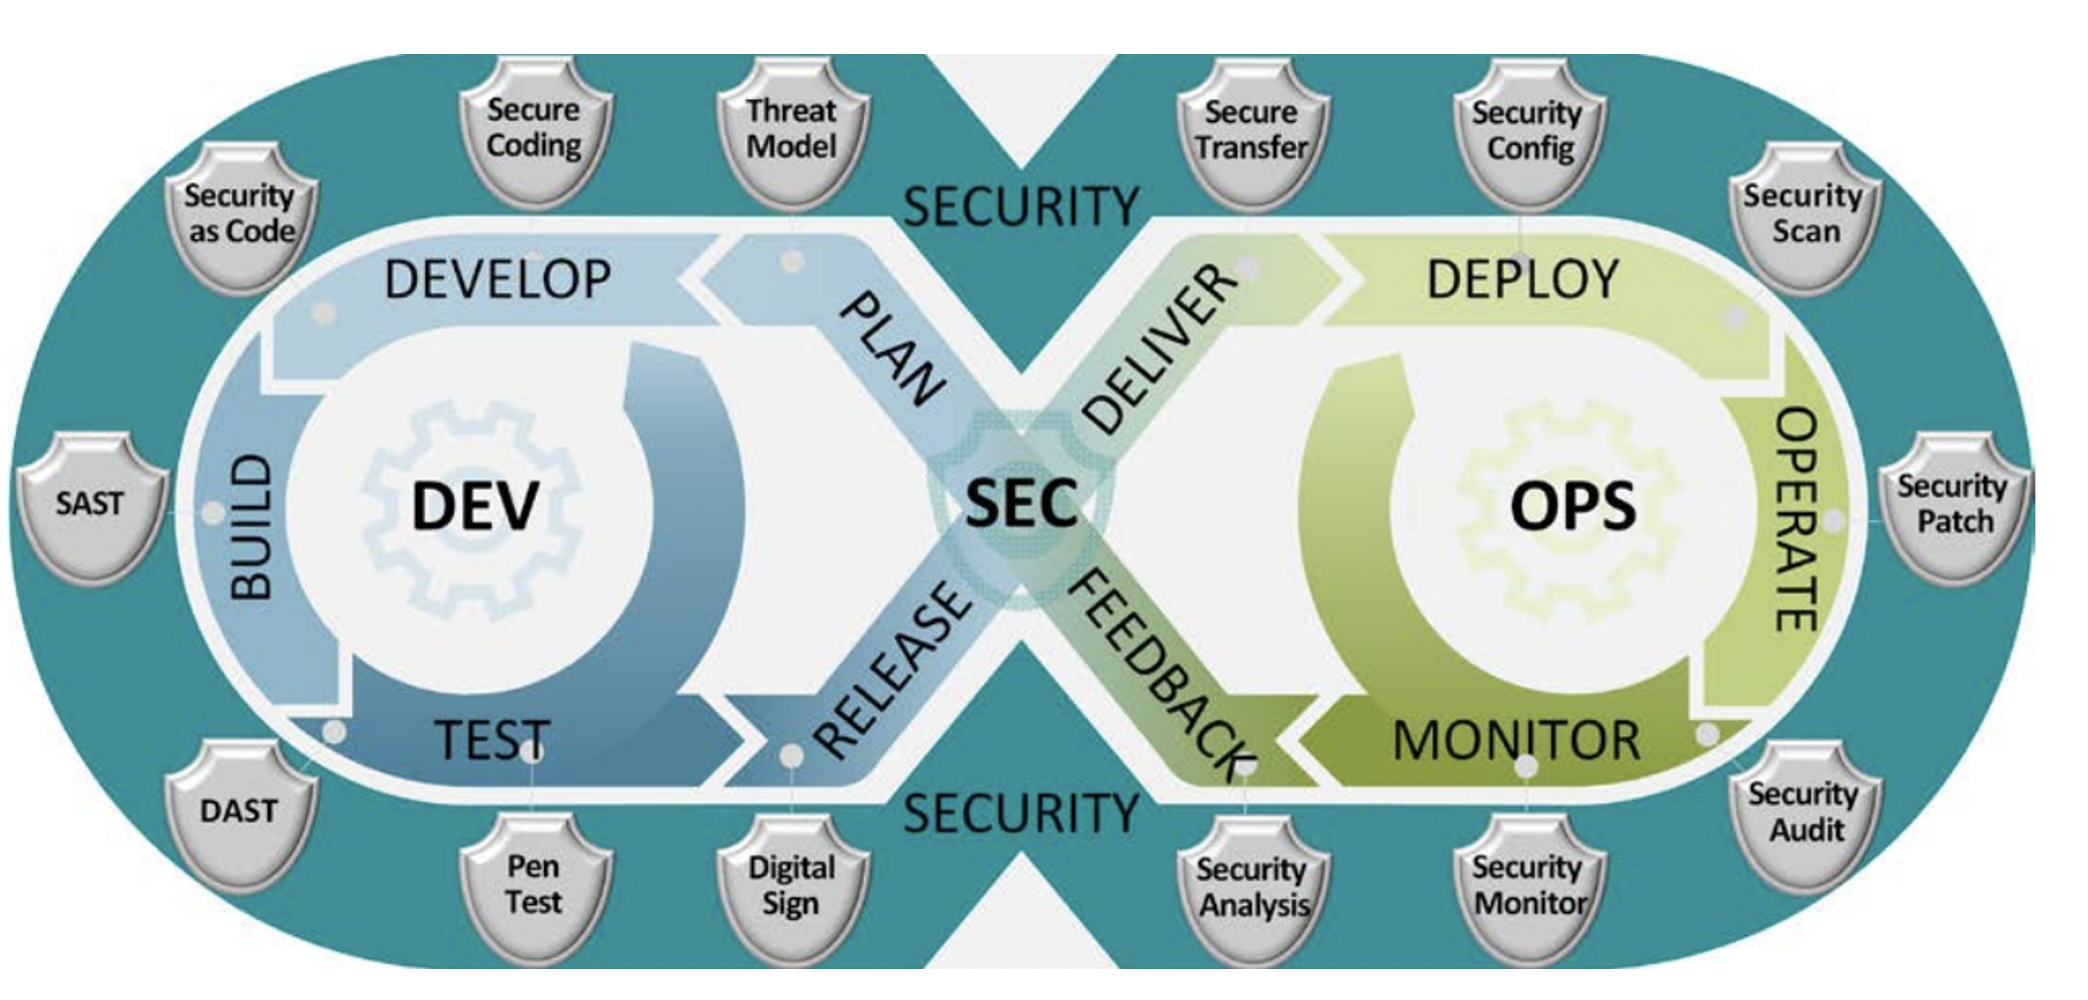
\includegraphics[width=0.8\textwidth,angle=00]{assets/f1.png}
\caption{Process overview}
\label{fig:processOverview}
\end{figure}


\paragraph{DevSecOPS Evangelist:} 
Usually the DevSecOPS team leader, he focuses on promoting the DevSecOPS advantages, identifying and quantifying companies’ benefits deriving from a higher agility. 

\paragraph{Release Manager:} 
The product stability manager which is basically the product owner. He cares about the product’s management and coordination. 

\paragraph{Automation Architect: }
Provides a complete automation role involving the DevSecOPS and Cloud solutions. He is an integration specialist that ensures the high availability of the pre-production and production systems. 

\paragraph{Software Developer/Tester:}
DevSecOPS developers are not responsible only for the transformation of new requirements into code, they also have to deal with testing, distribution and continuous monitoring processes.

\paragraph{Security Engineer: }
The DevSecOPS approach implements security by design.


\section*{Conclusion}

In this chapter, we started by introducing the project's background, highlighting the need for the project, and discussing the current state of the art. This was followed by a detailed description of the problem statement, which identifies the specific issue that the project aims to address. The ideation phase provided us with specific, measurable, achievable, relevant, and time-bound (SMART) objectives to ensure that they are attainable and can be evaluated. 

Overall, we gathered a rough understanding of the project's context, which is essential to understand the project's purpose, scope, and expected outcomes. It sets the foundation for the rest of the project and provides a clear roadmap for achieving the project's objectives.
\graphicspath{{./assets/}}
\setcounter{mtc}{2}
\chapter{Requirement analysis  }
\fancyhead[R]{\ungaramond\small\textbf{Chapter 2: Requirement analysis  }}
\minitoc
\newpage

\section*{Introduction}
In this chapter, our analysis is aimed at identifying the key actors in our design, the functional and non-functional needs our system is to provide for. We will then move on to an overview of the sprint bursts we have realized. Finally, we will provide a dissection of the ecosystem in the form of various UML diagrams. 

\section{Capturing requirements}
\subsection{Identifying key actors}
In this context, an actor is a user or any other system that interacts with the subject by exchanging signals and data.

\paragraph{Cloud architecture related actors:}
In order to have a devSecOPS compliant approach, it needs to be built on top of a containerized, highly available cloud infrastructure:
\begin{itemize}[label={--}]
\item Cloud architect: He is responsible for designing and implementing cloud computing solutions.
\item IaC tools: Although being a piece of software, it is necessary in order to automate provisioning and configuration of resources.
\item Cloud provider: Usually a third-party entity that allows for elastically allocating resources.
\item DevSecOPS team: A devSecOPS engineer is the consumer in this case, he uses the provisioned resources to build an ecosystem that is compliant with organizational needs.
\end{itemize}

\paragraph{CI/CD related actors:}
The cloud resources hold the value of a tool that is then leveraged to assist the development process:
\begin{itemize}[label={--}]
\item DevSecOPS team: uses the provisioned resources and follows an agile devSecOPS approach to build an ecosystem that is compliant with organizational needs.
\item Developer: A consumer of the devSecOPS ecosystem as well as the CI/CD workflow.
\item Company client: He is the end user and provides the specifications on software development.
\end{itemize}

\subsection{Functional requirements}

Formulating an understanding on functional requirements is a primordial phase in the implementation of the subject.

\begin{itemize}[label={--}]
\item A cloud-based infrastructure capable of hosting the devSecOPS ecosystem in terms of compute resources, storage and networking.
\item A continuous integration platform : The desired goal is to provide a CI workflow that channels the development effort in order to continuously ensure code quality.
\item A CD workflow: provide an automated and continuous delivery and deployment process.
\end{itemize}

\subsection{Non-functional requirements}

\begin{itemize}[label={--}]
\item High availability and resilience: Typically satisfied by distributed backend resources, orchestration and load balancing of workloads. 
\item Performance and scalability: Usually dependent on the cloud provider as well as the used technologies.
\item Security: An inbuilt quality that cloud and DevSecOPS offer by design.
\item Observability: A highly achievable need due the pluggability of containerized environments.
\item Usability: A somewhat hard to achieve requirement due to the rarity of a technologically adept workforce. 
\item Relatively low cost : the need to prioritize self-hosting and adopting opensource alternatives.
\end{itemize}


\section{Product backlog }

\subsection{Backlog history }
\begin{longtable}[H]{|m{1cm}|m{3cm}|m{1cm}|m{7cm}|m{1.2cm}|}
\hline
 {\textbf{Epic ID}} & {\textbf{EPIC}} & {\textbf{Story ID}} & {\textbf{Story}} & {\textbf{Prior-ity}} \\
 \hline
0 & \raggedright Certified devSecOps training &	0.1 &	Managing and running custom VMs. & \\
\cline{3-5}
&   & 0.2 &	Managing docker containers.	& \\
\cline{3-5}
&   & 0.3 &	CI/CD pipelines. & \\
\hline
1 & Maintenance and cleanup. &	1.1	& Exploring existing infrastructure and resources. & \\
\cline{3-5}
&   &	1.2 & Performing maintenance on enterprise assets. & \\

\hline
2 & Cloud design &	2.1 &	Information gathering phase. & \\
\hline
3 & Resource provisioning &	3.1 &	Provisioning resources using IaC playbooks. & \\
\hline
4 & Infrastructure setup. &	4.1 &	Infrastructure setup using IaC playbooks. & \\
\hline
5 & \raggedright Initial PaaS setup. &	5.1 &	Setting up ingress controller and TLS certificate provisioner.	 & \\
\cline{3-5}
&   & 5.2 &	Setting distributed storage backend.	 & \\
\cline{3-5}
&   & 5.3 &	Setting up network load balancer.	 & \\
  \hline
6 & Deployment of CI/CD platform &	6.1 &	Setting up personalized CI/CD orchestrator.	 & \\
\cline{3-5}
&   & 6.2 &	Setting up quality gate (CI).	 & \\
\cline{3-5}
&   & 6.3 & Setting up CD controller.	 & \\
  \hline
7 & \raggedright Preparation of automated CICD workflows. &	7.2 &	Structuring SCM backend	 & \\
\cline{3-5}
&   & 7.2 &	 \raggedright Using GitOPS and devOPS tools to automate CI/CD pipelines.	 & \\
   \hline
   
8 & \raggedright Deployment of authentication / authorization backend 	& 8.1 & \raggedright Self-managing distributed database storage backends (redis, mongoDB, postgresql).	 & \\
\cline{3-5}
&   & 8.2 &	\raggedright Deployment and configuration of authentication and authorization services.	 & \\
\cline{3-5}
&   & 8.3 &	\raggedright Configuring forward auth middlewares for secure access.	 & \\
   \hline
9 & \raggedright Implement a resilient disaster recovery strategy. & 9.1 &\raggedright  Provisioning cloud storage resources.		 & \\
\cline{3-5}
&   & 9.2 & \raggedright Preparing and applying backup strategy for application specific data.	 & \\
\cline{3-5}
&   & 9.3 &	\raggedright Preparing and applying backup strategy for PaaS specific workloads.	 & \\
 \hline
\caption{ Backlog History Table }
\end{longtable}
% \raggedright for space issue

\subsection{Sprint planning }
The project lasted seven months and a half starting on March 1st 2022. Overall, ten sprints have been followed with the typical duration of 3 weeks for each. 


\begin{longtable}[H]{|m{2cm}|m{10cm}|m{2cm}|}
\hline
 {\textbf{Sprint ID}} & {\textbf{Sprint Details }} & {\textbf{Duration }} \\ \hline 
0 
&
The first period was spent following a company sponsored devSecOps training. The following elements have been covered: 
Creating vm images using packer, spinning up virtual machines using vagrant,  
Using docker, docker compose plugin and docker container orchestration in swarm, 
An overview on CI/CD pipelines using Jenkins. 
&
4 weeks  \\
\hline
1 
&
The following three weeks were dedicated to exploring the existing infrastructure. Performing some maintenance and planning for migration. 
&
3 weeks  \\ \hline
2 
&
Next, we have started the information gathering phase in which we have formed an initial overview of the desired goals we would like to reach. 
&
2 weeks \\ \hline
3 
&
The use of IaC allowed us to provision the main cloud resources dedicated to hosting the PaaS infrastructure. 
&
2 weeks \\ \hline
4 
&
An initial setup of the provisioned resources was then automated and performed. 
&
3 weeks \\ \hline
5 
&
Putting in place the basic PaaS services, namely a distributed storage backend, a layer 2 load balancer, a cloud-native layer 4 ingress controller to route requests serving also as a reverse proxy and an application load balancer. 
&
3 weeks \\ \hline
6 
&
Mounting the backing CI/CD services which are mostly personalized to company needs. 
&
3 weeks \\ \hline
7 
&
Levering the CI/CD ecosystem to put in place pipelines to automate product testing, code quality checks, and delivery. 
&
4 weeks \\ \hline
8 
&
Securing access to company assets using an Authentication/Authorization middleware. 
&
3 weeks \\ \hline
9 
&
Putting in place a disaster recovery strategy that leverages distributed storage and S3 compliant object storage. 
&
3 weeks \\ \hline

\caption{Table Sprint planning}
\end{longtable}


\section{Modeling for cloud architecture and devops }

In order to facilitate collaboration and formulate an understanding of the system specifications and requirements, we have used the Unified Modeling Language (UML). 

\subsection{Cloud related diagrams }

\subsubsection{Class diagram of the provisioned cloud resources:}

\begin{figure}[H]\centering
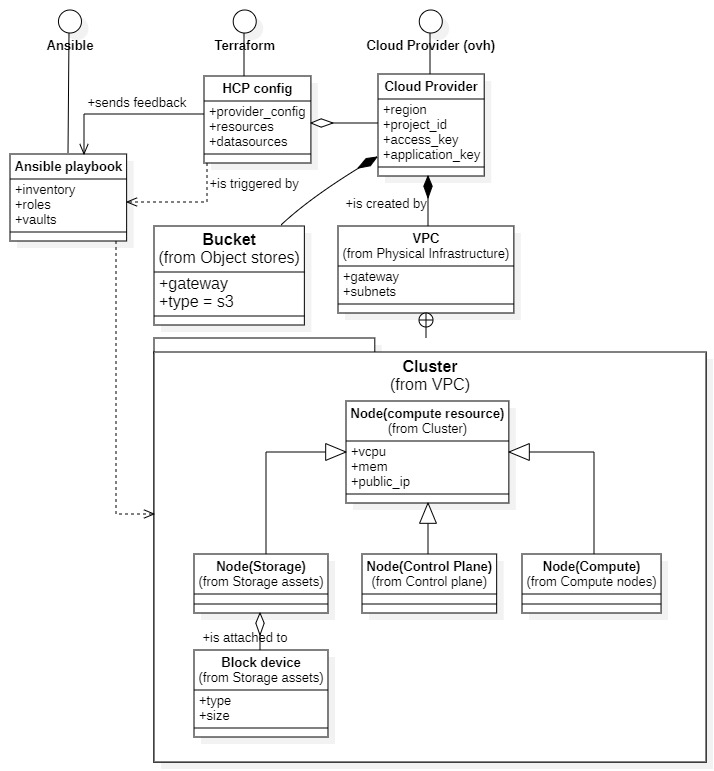
\includegraphics[width=1.0\textwidth,angle=00]{assets/f2.jpg}
\caption{Package diagram of the underlying cloud resources}
\label{fig:f2}
\end{figure}

\subsubsection{Sequence diagram for the provisioning and configuration:}

\begin{figure}[H]\centering
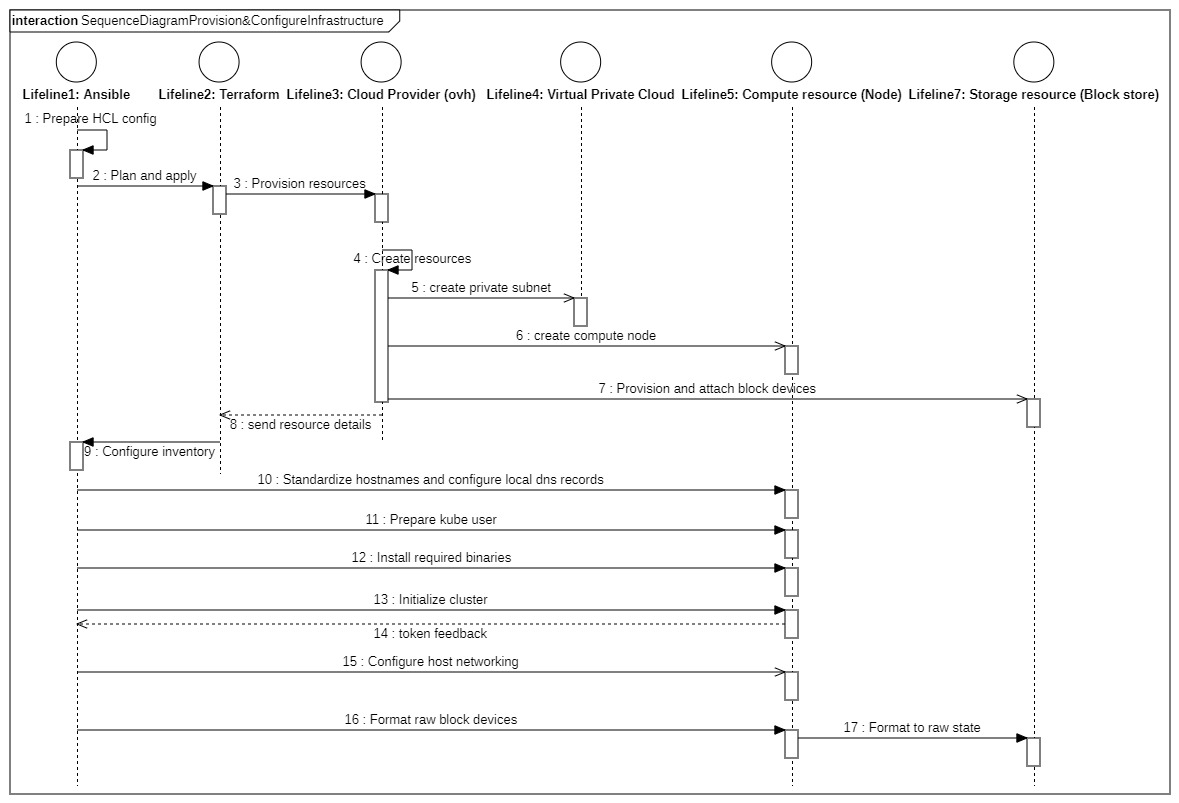
\includegraphics[width=1.0\textwidth,angle=00]{assets/f3.jpg}
\caption{Sequence diagram for the provisioning and configuration}
\label{fig:f3}
\end{figure}

\subsection{CI/CD related diagrams}

\subsubsection{Sequence diagram of a sample deployment: }

\begin{figure}[H]\centering
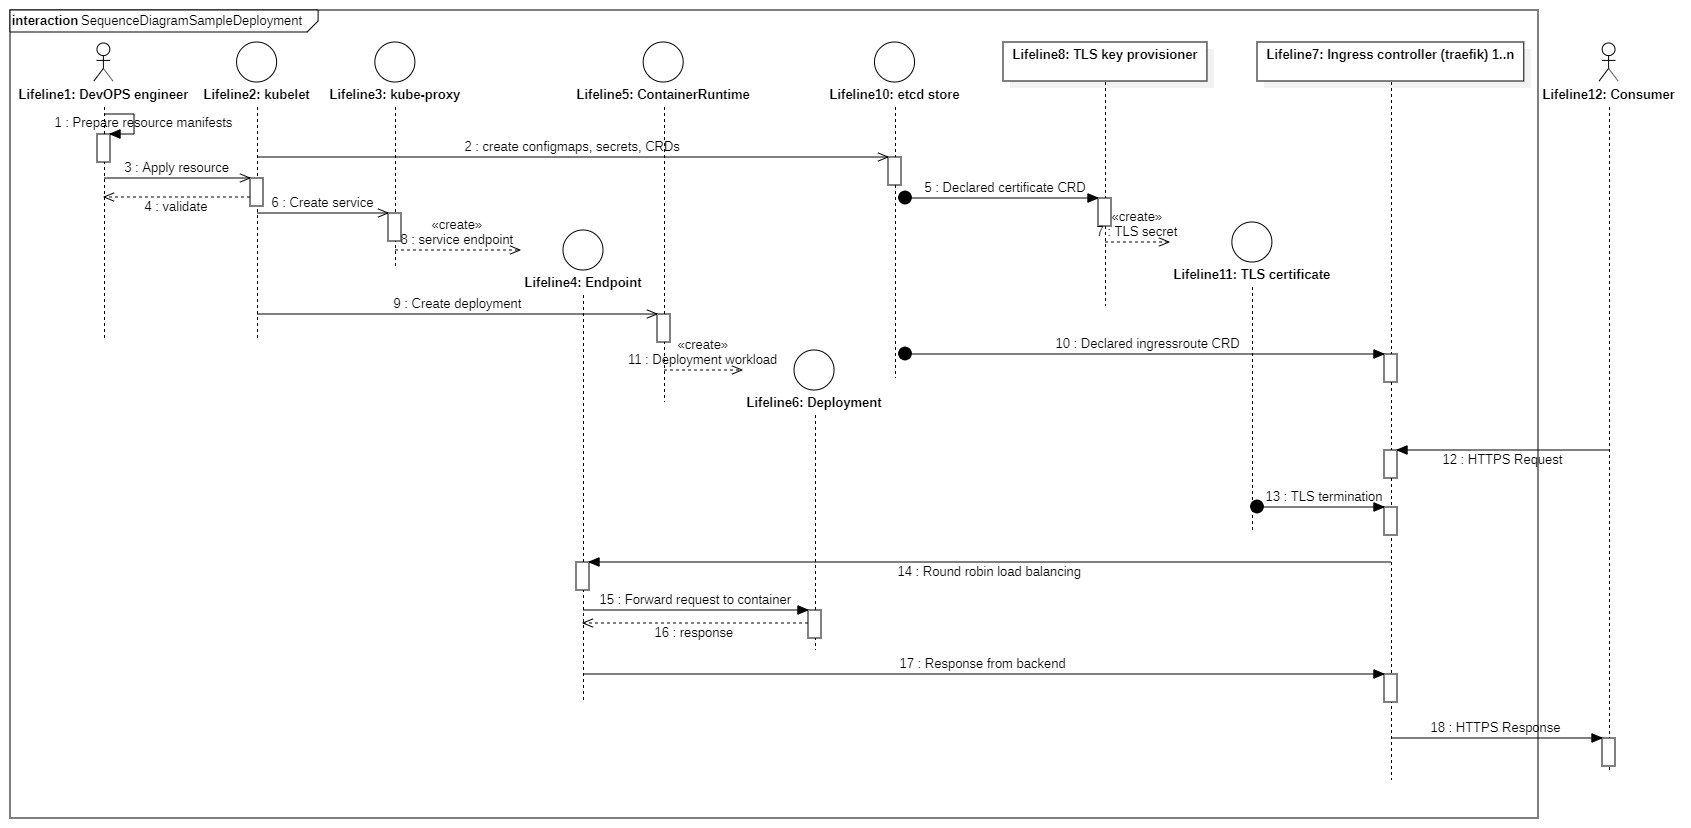
\includegraphics[width=1.0\textwidth,angle=00]{assets/f4.jpg}
\caption{Sequence diagram of a sample deploymen}
\label{fig:f4}
\end{figure}


\subsubsection{Sequence diagrams of the CI/CD workflow: }

\begin{figure}[H]\centering
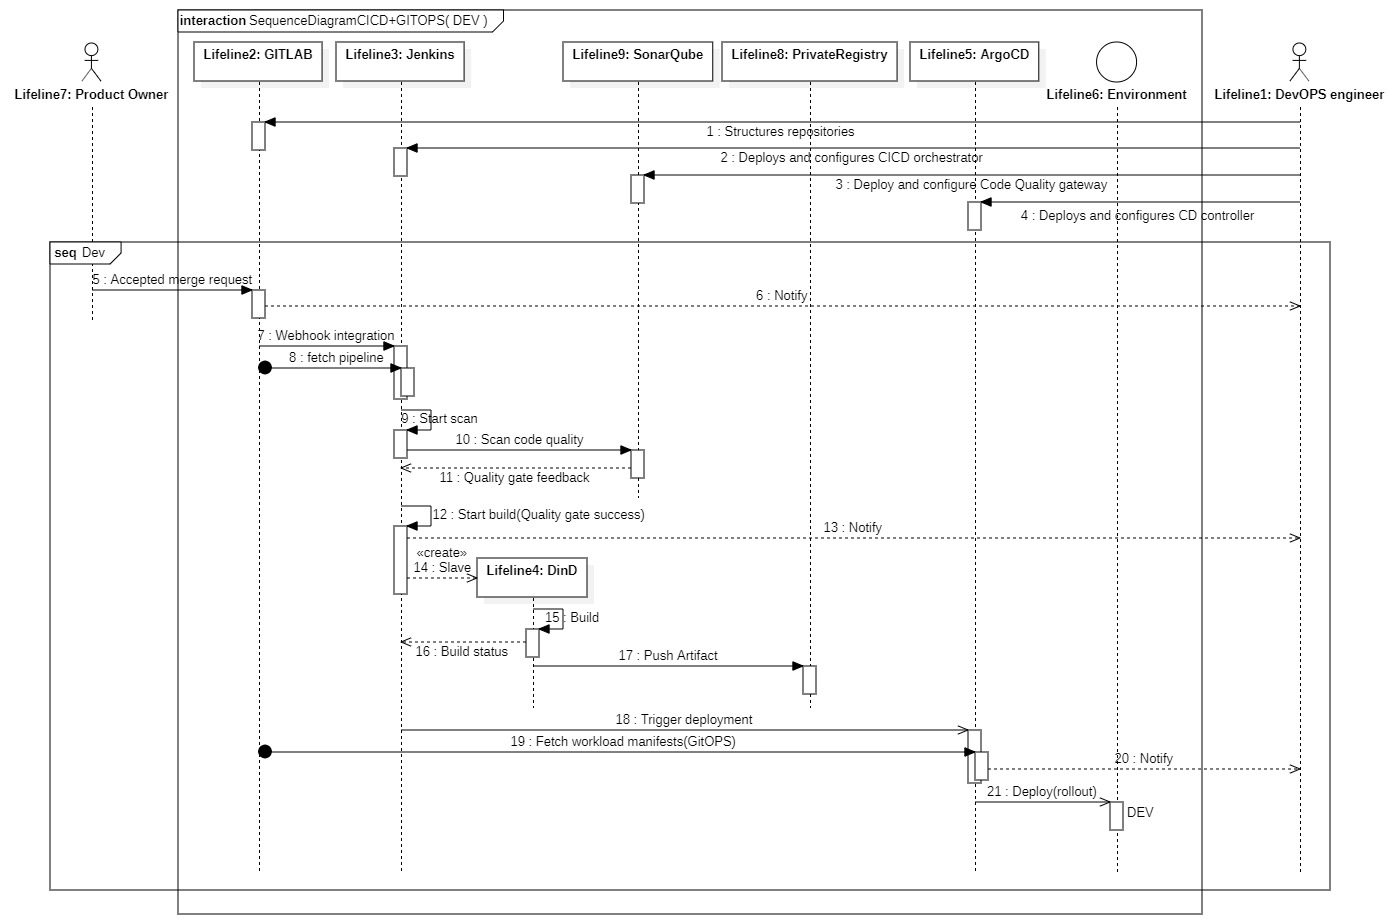
\includegraphics[width=1.0\textwidth,angle=00]{assets/f5.jpg}
\caption{Sequence diagrams of the CI/CD workflow in DEV}
\label{fig:f5}
\end{figure}

\begin{figure}[H]\centering
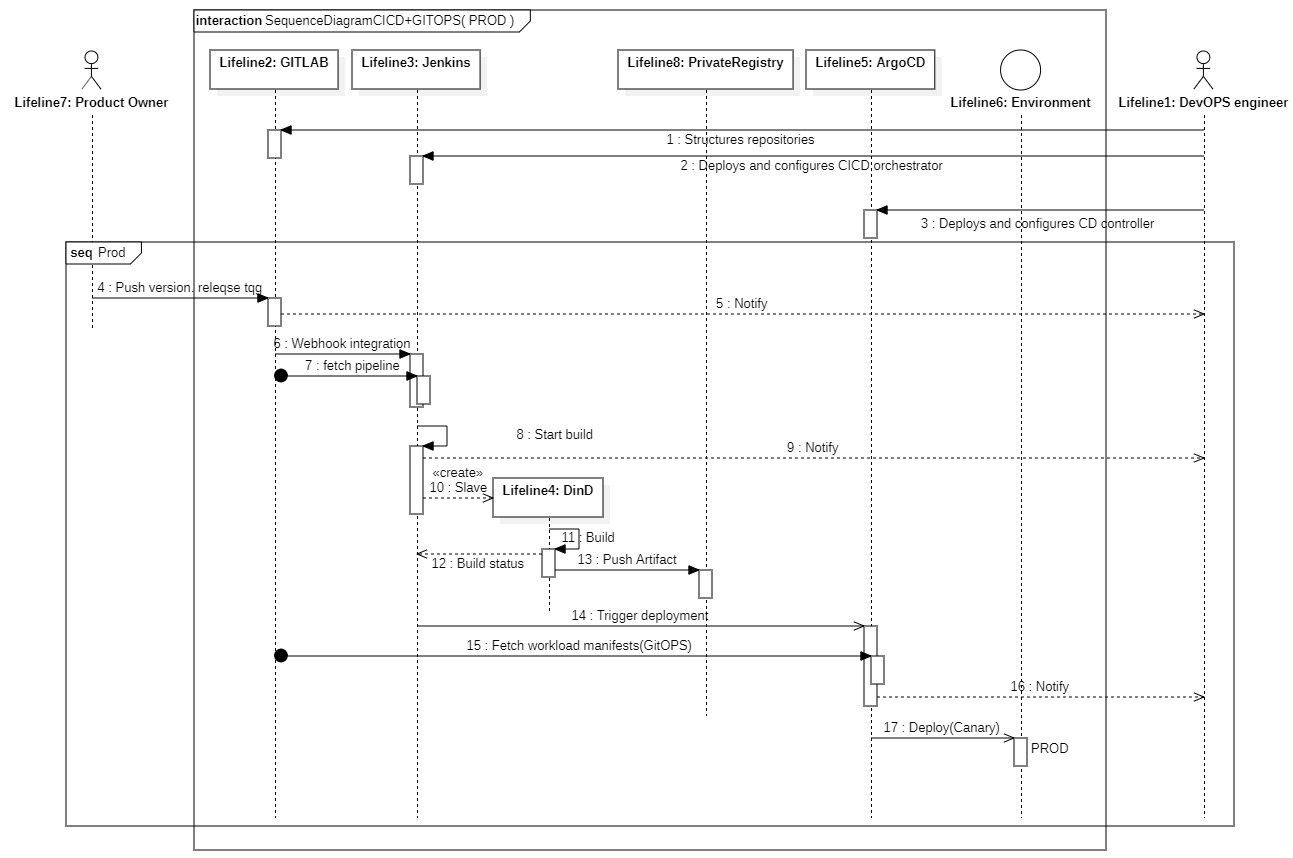
\includegraphics[width=1.0\textwidth,angle=00]{assets/f6.jpg}
\caption{Sequence diagrams of the CI/CD workflow in PROD}
\label{fig:f6}
\end{figure}


\subsection{Technological choices }
% \paragraph{Development tools }
In this section, we layout the cloud provider choice,
\subsubsection{Cloud provider choice: } 

\paragraph{OVH : }

A decisive factor concerning the cloud provider choice is related to company’s desire to opt mainly for a provider that is based in France.  

\paragraph{Openstack: }

OVH uses openstack as its backing cloud computing infrastructure. Thus, conversing with components as neutron, nova, glance, swift is a must. 

\subsubsection{Infrastructure as code tools }

\paragraph{Terraform: }

An industry standard for conversing with cloud providers in order to provision and configure resources. 

\paragraph{Ansible: }

We have opted for ansible because it’s faster than its alternatives namely chef, and easier to use.  

\subsubsection{Containerization and orchestration techniques: }

\paragraph{Container orchestrator: Kubernetes v1.21 }

An open source container orchestration tool that automates the deployment, scaling, and managing containerized applications. 

\paragraph{Container runtime : containerd }

A daemon for linux that manages the complete container lifecycle. 

\paragraph{Container platform : docker-ce v20.10 }

The container management tool that uses containerd to manage container lifecycles and their underlying abstractions such as volumes and networking.  

\paragraph{Container networking: Calico }

A cloud-native plugin deployment in Kubernetes that uses the CNI API to provide a networking and security solution in the cluster. 

\paragraph{Container platform : docker-ce v20.10 }

The container management tool that uses containerd to manage container lifecycles and their underlying abstractions such as volumes and networking. 

\paragraph{Container networking: Calico }

A cloud-native plugin deployment in Kubernetes that uses the CNI API to provide a networking and security solution in the cluster. 


\subsubsection{Self-hosted PaaS services }

\paragraph{Distributed storage backend: Ceph }

A highly reliable, open source, distributed storage platform offering bloc , filesystem and object storage volumes to be leveraged by the orchestrator. 

\paragraph{Ingress Controller: Traefik ingress controller }

An open-source edge router serving as an ingress controller, a reverse proxy and a load balancer. 

\paragraph{Layer 2 load balancer: MetalLB }

This opensource load balancer provides support for bare metal Kubernetes clusters using standard protocols. 

\paragraph{Private registry: harbor }

An open-source private registry serving as a backend to sore artifacts in a secure manner. 

\paragraph{Database storage (document): Redis, MongoDB }

Database storage in document format is provided by a replicated mongoDB cluster. An in memory redis cluster allows for session storage. 

\paragraph{Database storage (SQL): PostgreSQL }

A PostgreSQL cluster in HA mode coupled with a PGpool middleware to distribute load and control replication. 

\paragraph{Authentication middleware: Authelia }

An open-source portal serving as an authentication and authorization server. It leverages the “forward auth” capability of the ingress controller to regulate access. 

\paragraph{User management: OpenLDAP }

An open-source implementation of the Lightweight Directory Access Protocol that is used to manage organizational user credentials and details. 

\paragraph{SCM tool: Gitlab }

An enterprise solution for source code management and versioning. 

\paragraph{CI/CD orchestration: Jenkins }

An open-source automation server which enables build, test, and deployment processes. 

\paragraph{Quality gate: SonarQube }

An open-source platform that allows for continuous inspection of code quality. 

\paragraph{CD controller: ArgoCD, ArgoRollouts }

An open-source declarative, GitOPS continuous delivery tool for Kubernetes. 

\paragraph{Disaster recovery: Velero }

An open-source tool to safely backup and restore, perform disaster recovery, and migrate Kubernetes cluster resources and persistent volumes. 

\paragraph{Config formats: YAML, TOML, HCP config, JSON }

\subsubsection{Development tools }

\paragraph{Development IDE: VS Code }

A pluggable, lightweight opensource IDE. 

\paragraph{SSH platform: Termius }

A platform that offers port forwarding and secure file transfer over ssh. 

\subsubsection{Development languages }

\paragraph{Scripting: python, shell, groovy }

Shell was used to interface with the linux operating system. For conversing with APIs, an assortment of python scripts were developed to automate various tasks, namely, database backups. Jenkins pipelines and configurations were written in groovy. 

\paragraph{Templating: YTT, jinja2 }

To template various configuration files that are dependent on the deployment environment, we used YTT for YAML/JSON. Jinja2 was the main templating tool for ansible playbooks. 

\section{Architectural specifications}

\subsection{Physical architecture}

The following figure is an overview of the infrastructure resource setup:

\begin{figure}[H]\centering
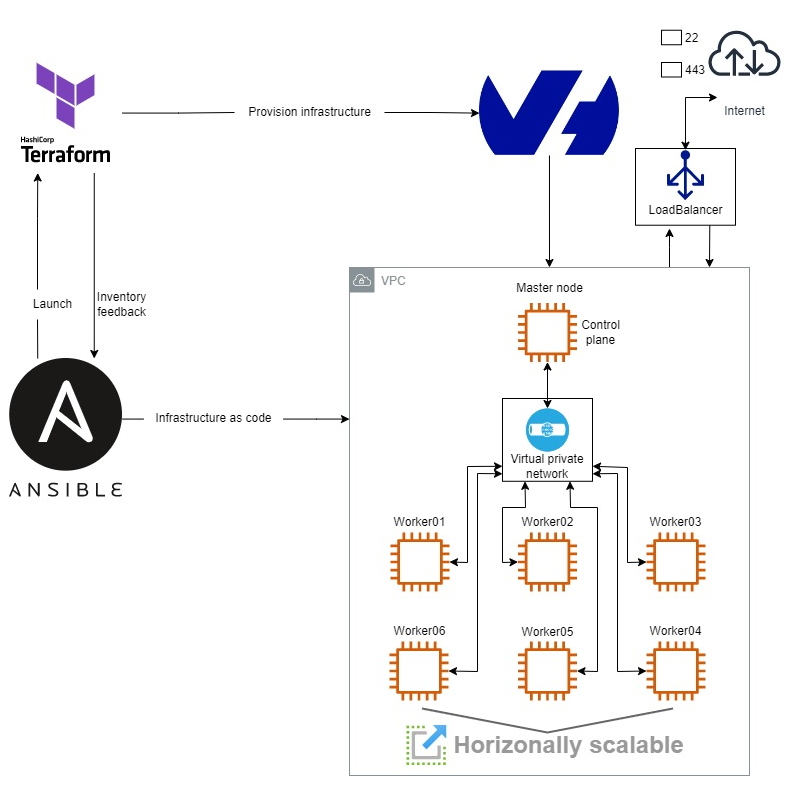
\includegraphics[width=1.0\textwidth,angle=00]{assets/f7.jpg}
\caption{Physical architecture}
\label{fig:f7}
\end{figure}

\subsection{PaaS deployment architecture} 
Next we layout the organization of the subsystems, software classes, and layers that make the complete logical system of our PaaS infrastructure :

\begin{figure}[H]\centering
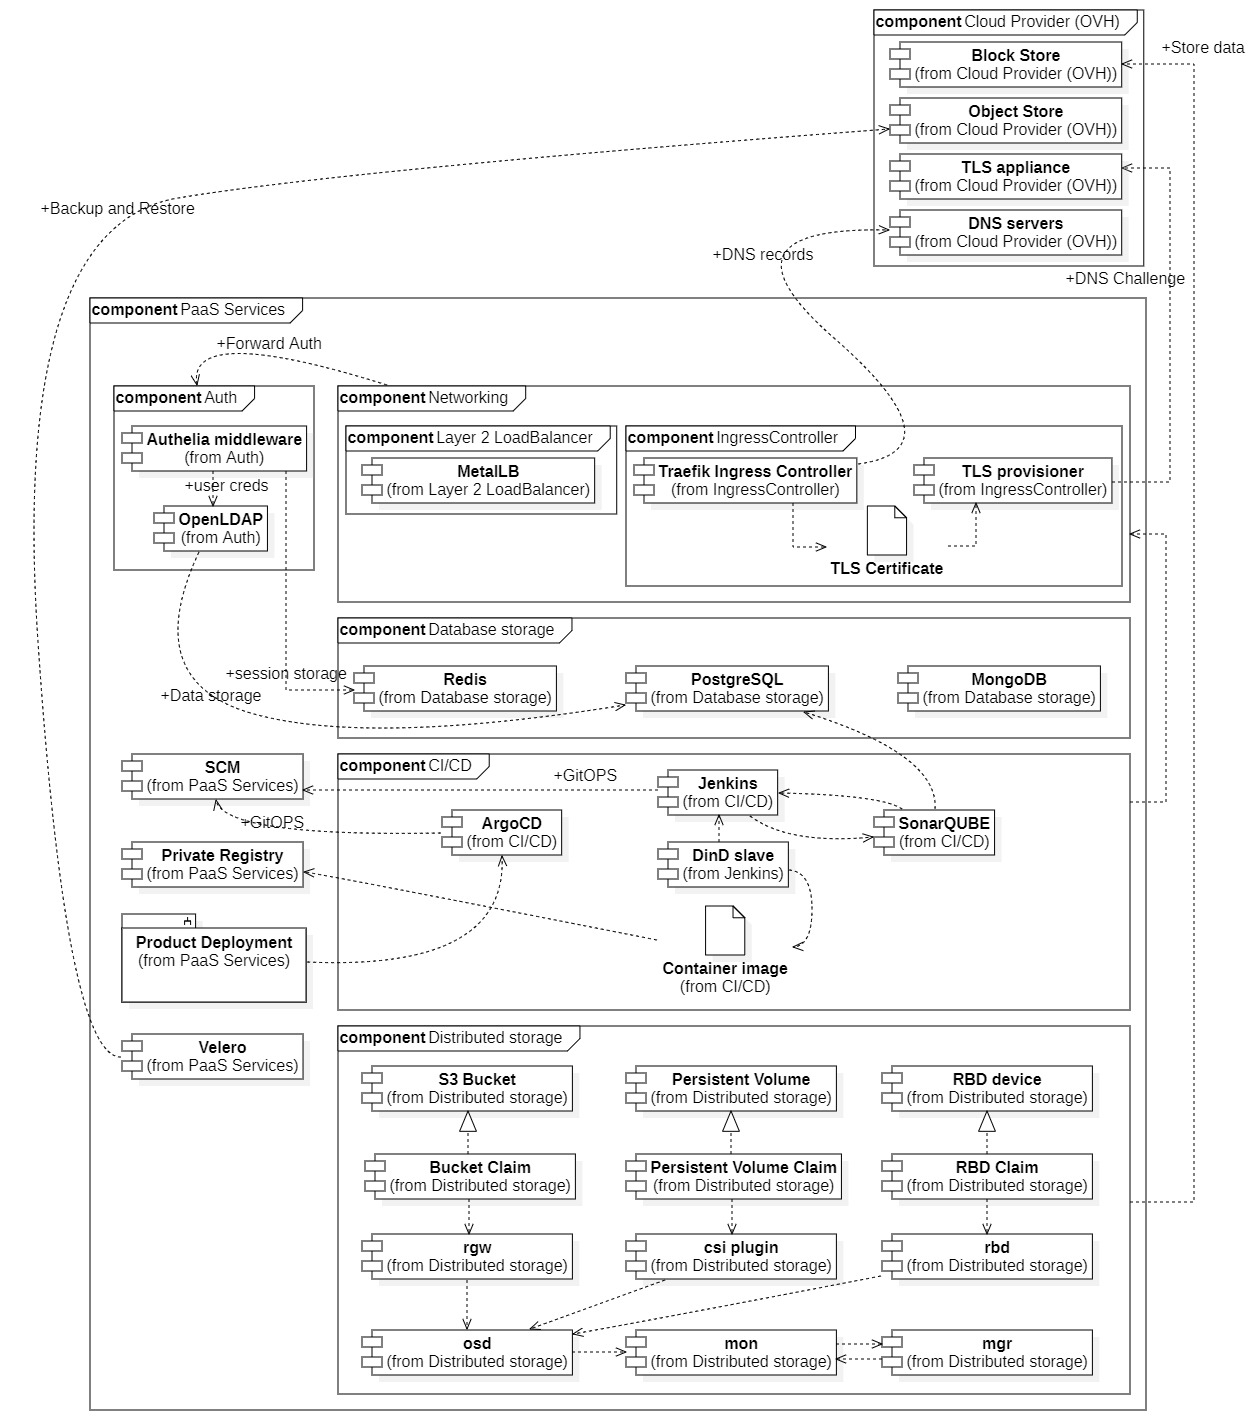
\includegraphics[width=1.0\textwidth,angle=00]{assets/f8.jpg}
\caption{PaaS infrastructure}
\label{fig:f8}
\end{figure}

\section{Workspace description}

To implement the project, the company has provided us with the necessary hardware equipment, certified preliminary training as well as the desired cloud resources.

\section*{Conclusion}
All the functional and non-functional requirements have been viewed in this chapter through the use of package, class and sequence diagrams. We have also formed an understanding on the underlying resources and services through the physical architecture and the PaaS deployment diagram.



\graphicspath{{./assets/}}
\setcounter{mtc}{3}
\chapter{1st Sprint: Maintenance of existing resources  }
\fancyhead[R]{\ungaramond\small\textbf{Chapter III. 1st Sprint: Maintenance of existing resources }}
\minitoc
\newpage


\section*{Introduction}
The first sprint was dedicated towards exploring the existing services and resources, performing some minor changes and putting in place a backup strategy.

\section{Sprint backlog :}



\begin{longtable}[!ht]{|m{1.5cm}|m{3cm}|m{1.5cm}|m{9cm}|}
\hline
{\textbf{EpicID}} & {\textbf{Epic}} & {\textbf{StoryID}} & {\textbf{Story}} \\
\hline
1 &  \raggedright Exploring assets.	& 1.1  & SCM structuring: service components need to be split into different repos. \\
\cline{3-4}
& & 1.2 &  	Keeping track of developed applications and their requirements \\
\hline
2  & Maintenance. &	2.1	 &  Rebuilding optimized containers for developed applications. \\
\cline{3-4}
& & 2.2 & Backup of existing data on current infrastructure in S3 containers.\\
\hline
\end{longtable}

\section{Maintenance operations}
\paragraph{}
In this sprint, we have assembled standalone self-hosted services into a single stack of upgraded container versions in order to provide better visibility of workloads. A container management platform was then added to this stack to improve on operability. 
The following figure is the deployment diagram of the resulting docker-compose stack:

 \begin{figure}[!ht]\centering
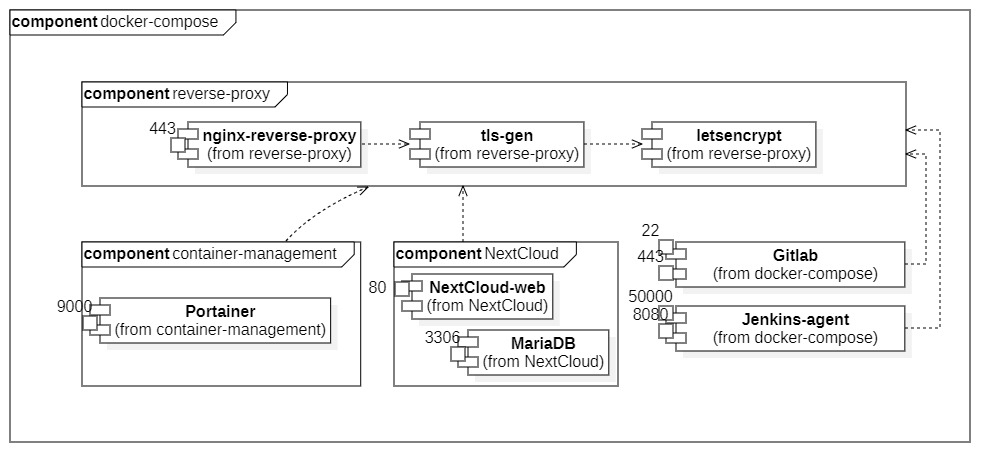
\includegraphics[width=0.8\textwidth,angle=00]{assets/f9.jpg}
\caption{PaaS infrastructure}
\label{fig:f9}
\end{figure}

\section{Application overview and SCM structuring.}

\paragraph{}
Two main applications were in development during this project. We have recommended a better source code management strategy that resulted in separating services into different repos in order to optimize the container image creation process. The resulting deployment diagram Is as follows:
 
\section*{Conclusion}
\paragraph{}In this chapter we have successfully performed



% Introduction
% In this chapter, our analysis is aimed at identifying the key actors in our design, the functional and non-functional needs our system is to provide for. We will then move on to an overview of the sprint bursts we have realized. Finally, we will provide a dissection of the ecosystem in the form of various UML diagrams.
% \section{Capturing requirements}
% \subsection{Identifying key actors}
% In this context, an actor is a user or any other system that interacts with the subject by exchanging signals and data.
% \subsubsection*{Cloud architecture related actors:}
% In order to have a devSecOPS compliant approach, it needs to be built on top of a containerized, highly available cloud infrastructure:
% \newline
% -	Cloud architect: He is responsible for designing and implementing cloud computing solutions.
% \newline
% -	IaC tools: Although being a piece of software, it is necessary in order to automate provisioning and configuration of resources.
% \newline
% -	Cloud provider: Usually a third-party entity that allows for elastically allocating resources.
% \newline
% -	DevSecOPS team: A devSecOPS engineer is the consumer in this case, he uses the provisioned resources to build an ecosystem that is compliant with organizational needs.
% \subsubsection*{CI/CD related actors:}
% The cloud resources hold the value of a tool that is then leveraged to assist the development process:
% \newline
% -	DevSecOPS team: uses the provisioned resources and follows an agile devSecOPS approach to build an ecosystem that is compliant with organizational needs.
% \newline
% -	Developer: A consumer of the devSecOPS ecosystem as well as the CI/CD workflow.
% \newline
% -	Company client: He is the end user and provides the specifications on software development.

% \subsection{Functional requirements}

% Formulating an understanding on functional requirements is a primordial phase in the implementation of the subject.
% \newline
% -	A cloud-based infrastructure capable of hosting the devSecOPS ecosystem in terms of compute resources, storage and networking.
% \newline
% -	A continuous integration platform : The desired goal is to provide a CI workflow that channels the development effort in order to continuously ensure code quality.
% \newline
% -	A CD workflow: provide an automated and continuous delivery and deployment process.

% \subsection{Non-functional requirements}
% -	High availability and resilience: Typically satisfied by distributed backend resources, orchestration and load balancing of workloads. \newline
% -	Performance and scalability: Usually dependent on the cloud provider as well as the used technologies.\newline
% -	Security: An inbuilt quality that cloud and DevSecOPS offer by design.\newline
% -	Observability: A highly achievable need due the pluggability of containerized environments.\newline
% -	Usability: A somewhat hard to achieve requirement due to the rarity of a technologically adept workforce. \newline
% -	Relatively low cost : the need to prioritize self-hosting and adopting opensource alternatives.

% \newpage
% \section{Product backlog }

% \subsection{Backlog history }

% \begin{longtable}[!ht]{|m{1cm}|m{3cm}|m{1cm}|m{7cm}|m{1.2cm}|}
% \hline
%  {\textbf{Epic ID}} & {\textbf{EPIC}} & {\textbf{Story ID}} & {\textbf{Story}} & {\textbf{Prior-ity}} \\
%  \hline
% 0 & \raggedright Certified devSecOps training &	0.1 &	Managing and running custom VMs. & \\
% \cline{3-5}
% &   & 0.2 &	Managing docker containers.	& \\
% \cline{3-5}
% &   & 0.3 &	CI/CD pipelines. & \\
% \hline
% 1 & Maintenance and cleanup. &	1.1	& Exploring existing infrastructure and resources. & \\
% \cline{3-5}
% &   &	1.2 & Performing maintenance on enterprise assets. & \\

% \hline
% 2 & Cloud design &	2.1 &	Information gathering phase. & \\
% \hline
% 3 & Resource provisioning &	3.1 &	Provisioning resources using IaC playbooks. & \\
% \hline
% 4 & Infrastructure setup. &	4.1 &	Infrastructure setup using IaC playbooks. & \\
% \hline
% 5 & \raggedright Initial PaaS setup. &	5.1 &	Setting up ingress controller and TLS certificate provisioner.	 & \\
% \cline{3-5}
% &   & 5.2 &	Setting distributed storage backend.	 & \\
% \cline{3-5}
% &   & 5.3 &	Setting up network load balancer.	 & \\
%   \hline
% 6 & Deployment of CI/CD platform &	6.1 &	Setting up personalized CI/CD orchestrator.	 & \\
% \cline{3-5}
% &   & 6.2 &	Setting up quality gate (CI).	 & \\
% \cline{3-5}
% &   & 6.3 & Setting up CD controller.	 & \\
%   \hline
% 7 & \raggedright Preparation of automated CICD workflows. &	7.2 &	Structuring SCM backend	 & \\
% \cline{3-5}
% &   & 7.2 &	 \raggedright Using GitOPS and devOPS tools to automate CI/CD pipelines.	 & \\
%    \hline
%    \newpage
%      \hline
% 8 & \raggedright Deployment of authentication / authorization backend 	& 8.1 & \raggedright Self-managing distributed database storage backends (redis, mongoDB, postgresql).	 & \\
% \cline{3-5}
% &   & 8.2 &	\raggedright Deployment and configuration of authentication and authorization services.	 & \\
% \cline{3-5}
% &   & 8.3 &	\raggedright Configuring forward auth middlewares for secure access.	 & \\
%    \hline
% 9 & \raggedright Implement a resilient disaster recovery strategy. & 9.1 &\raggedright  Provisioning cloud storage resources.		 & \\
% \cline{3-5}
% &   & 9.2 & \raggedright Preparing and applying backup strategy for application specific data.	 & \\
% \cline{3-5}
% &   & 9.3 &	\raggedright Preparing and applying backup strategy for PaaS specific workloads.	 & \\
%  \hline
% 10	& \raggedright Load testing, benchmarking.& 10.1 & Load testing and benchmarking of assets. & \\	
% \hline

% \end{longtable}
% % \raggedright for space issue

% \newpage
% \subsection{Sprint planification }
% The project lasted seven months and a half starting in March, 1st 2022. Overall ten sprints have been followed with the typical duration of 3 weeks for each. 


% \begin{table}[h!]
% \center
% \begin{tabular}[b]{|m{3cm}|m{8cm}|m{2cm}|}
% \hline
%  {\textbf{Sprint ID}} & {\textbf{Sprint Details }} & {\textbf{Duration }} \\ \hline 
% 0 
% &
% The first period was spent following a company sponsored devSecOps training. The following elements have been covered: 
% Creating vm images using packer, spinning up virtual machines using vagrant,  
% Using docker, docker compose plugin and docker container orchestration in swarm, 
% An overview on CI/CD pipelines using Jenkins. 
% &
% 4 weeks  \\
% \hline
% 1 
% &
% The following two weeks were dedicated to exploring the existing infrastructure. Performing some maintenance and planning for migration. 
% &
% 3 weeks  \\ \hline
% 2 
% &
% Next, we have started the information gathering phase in which we have formed an initial overview of the desired goals we would like to reach. 
% &
% 2 weeks \\ \hline
% 3 
% &
% The use of IaC allowed us to provision the main cloud resources dedicated to hosting the PaaS infrastructure. 
% &
% 2 weeks \\ \hline
% 4 
% &
% An initial setup of the provisioned resources was then automated and performed. 
% &
% 3 weeks \\ \hline
% 5 
% &
% Putting in place the basic PaaS services, namely a distributed storage backend, a layer 2 load balancer, a cloud-native layer 4 ingress controller to route requests serving also as a reverse proxy and an application load balancer. 
% &
% 3 weeks \\ \hline
% 6 
% &
% Mounting the backing CI/CD services which are mostly personalized to company needs. 
% &
% 3 weeks \\ \hline
% 7 
% &
% Levering the CI/CD ecosystem to put in place pipelines to automate product testing, code quality checks, and delivery. 
% &
% 4 weeks \\ \hline
% 8 
% &
% Securing access to company assets using an Authentication/Authorization middleware. 
% &
% 3 weeks \\ \hline
% 9 
% &
% Putting in place a disaster recovery strategy that leverages distributed storage and S3 compliant object storage. 
% &
% 3 weeks \\ \hline
% 10 
% &
% Assessing the performance of the PaaS put in place and planning to enhancements 
% &
% 2 weeks \\ \hline
% \end{tabular}
% \caption{Table Sprint planification}
% \textcolor{white}{I} \label{tab:tab-m}
% \end{table}

% \section{Modeling for cloud architecture and devops }
% \subsection{Class diagram for cloud architecture }

% \subsection{Technological choices }
% \subsubsection*{Development tools }

% \newpage
% \subsubsection*{Infrastructure as code tools  }

% \subsubsection*{Containerization and orchestration techniques  }
% \subsubsection*{Self-hosted paas services }
% \subsubsection*{Cloud provider choice}


% \section*{Conclusion}

\graphicspath{{./assets/}}
\setcounter{mtc}{4}
\chapter{2nd Sprint: Information gathering and cloud design }
\fancyhead[R]{\ungaramond\small\textbf{Chapter IV. 2nd Sprint: Information gathering and cloud design }}
\minitoc
\newpage

\section*{Introduction}
\section{Sprint backlog :}

\begin{longtable}[!ht]{|m{1.5cm}|m{3cm}|m{1.5cm}|m{9cm}|}
\hline
{\textbf{Epic ID}} & {\textbf{Epic}} & {\textbf{Story ID}} & {\textbf{Story}}\\
\hline
1  & Information gathering.	 &  1.1	 &  esearch provider specific (OVH) constraints\\
\cline{3-4}
& & 1.2 & Container orchestration choice. \\
\cline{3-4}
& & 1.3	& Deciding on virtualized networking. \\
\cline{3-4}
& & 1.4	& Deciding on application load balancer. \\
\cline{3-4}
& & 1.5	& Deciding on network level load balancer. \\
\cline{3-4}
& & 1.6	& Storage backend choice.\\
\hline
\end{longtable}


\section{Package diagram of cloud resources :}

The cluster resources are basically cloud instances with different specifications tailored to their use cases. Three major groups of resources are distinguished in the following diagram: Control plane instances, Compute instances and storage assets which are object store buckets and compute instances to which raw block stores are attached.

\begin{figure}[!ht]\centering
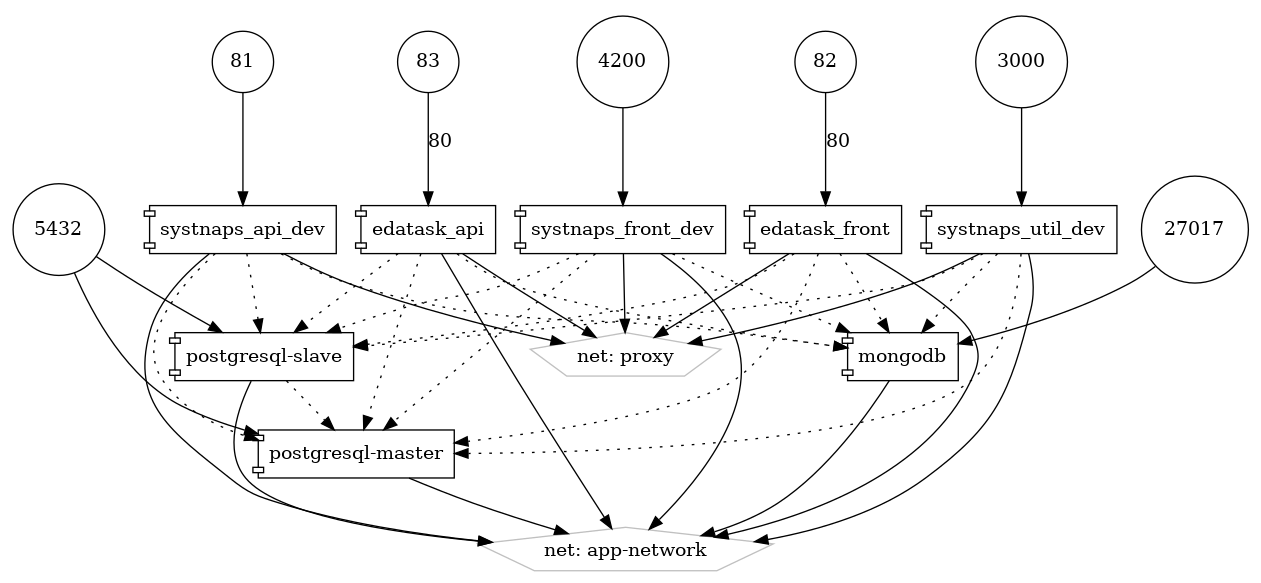
\includegraphics[width=0.8\textwidth,angle=00]{assets/f10.png}
\caption{Package diagram of cloud resources }
\label{fig:f10}
\end{figure}

\newpage
Comparative study on container orchestration: 

Container Orchestration Engines such as “Kubernetes”, “Apache mesos” and “docker swarm” are platforms for managing containers and automating the deployment, scaling, and operations of containers across a cluster of nodes. This is achieved by pooling the discrete cloud resources into a single PaaS on which deployments can be deployed. 

\begin{table}[h!]
\center
\begin{tabular}[b]{|m{3cm}|m{4cm}|m{4cm}|m{4cm}|}
\hline
Criteria & Kubernetes & Docker swarm & Apache Mesos  \\
\hline
Ease of use & Medium & Easy & Complex  \\
\hline
Cluster scalability & Medium to Large & Small to Medium & Very Large  \\
\hline
Cluster installation & Complex & Easy & Medium  \\
\hline
Container deployment & YAML based  & Docker based & JSON based \\
\hline
\end{tabular}
\caption{Table Sprint planification}
\textcolor{white}{I} \label{tab:tab-m}
\end{table}

\paragraph{}Kubernetes is our container orchestration tool of choice in this project. We envision to take on the challenge of putting in place a complete sustainable PaaS by leveraging its adaptability through the use of custom resource definitions. 


\section{Package diagram for the PaaS logical components:}

\begin{figure}[!ht]\centering
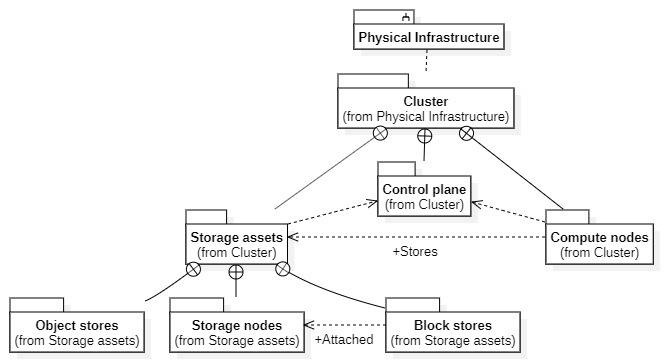
\includegraphics[width=0.8\textwidth,angle=00]{assets/f11.jpg}
\caption{Package diagram for the PaaS logical components}
\label{fig:f11}
\end{figure}


\paragraph{}This figure illustrates a package design of the main PaaS services. We mainly distinguish :\newline
-	A control plane: which manages assets in the cluster, namely, nodes, pods and other api resources. \newline
-	An assortment of networking services which allow for ingress control in both the network and application layers.\newline
-	An authentication and authorization service: which is aimed to control access to the cluster.\newline
-	A distributed, scalable, and replicated storage backend which is independent of the infrastructure in place to provide data redundancy and disaster recovery.

\section*{Conclusion}

% \section*{Introduction}
% Nous continuons la phase de réalisation de ce projet par le deuxième sprint où on va se focaliser sur le développement de la partie backend ainsi que la communication avec le moteur graphique en les détaillant par la backlog produit et le diagramme de cas d’utilisation raffiné pour chaque cas d’utilisation pour finir avec quelques captures d’écran de chaque cas d’utilisation.

% \section{Sprint  Backlog}
% \subsection{Histoires\textcolor{white}{J}\`a\textcolor{white}{J}r\'ealiser}

% La\textcolor{white}{J}liste\textcolor{white}{J}des\textcolor{white}{J}tâches\textcolor{white}{J}à\textcolor{white}{J}réaliser\textcolor{white}{J}dans\textcolor{white}{J}le\textcolor{white}{J}sprint\textcolor{white}{J}deux est\textcolor{white}{J}décrite\textcolor{white}{J}dans\textcolor{white}{J}le\textcolor{white}{J}tableau \ref{tab:sprint_4_backlog} \textcolor{white}{J}.

% \begin{longtable}[!ht]{|m{1cm}|m{3cm}|m{1cm}|m{7cm}|m{1.3cm}|}
% \hline
% {\textbf{Id story}} & {\textbf{User story}} & {\textbf{id tâche}} & {\textbf{tâche}} & {\textbf{estima-tion(H)}}\\
% \hline
% 1.1 & En tant qu’utilisateur je souhaite sauvegarder la session  & 1.1.1 & Initiation et configuration des projets de la partie backend & 6\\
% \cline{3-5}
% &   & 1.1.2 & Mise en place de l’architecture cible & 2\\
% \cline{3-5}
% &	& 1.1.3 & Développement de la partie Backend & 8\\
% \cline{3-5}
% &	& 1.1.4 & Communication avec le moteur graphique & 4\\
% \cline{3-5}
% &	& 1.1.5 & Intégration du protocole d’autorisation OAuth2 & 10\\
% \cline{3-5}
% &	& 1.1.6 & Validation du token et renvoie des images au client & 10\\
% \cline{3-5}
% &	& 1.1.7 & Configuration de la base de données No SQL Cosmos DB & 1\\
% \cline{3-5}
% &	& 1.1.8 & Connecter la partie backend a la base de données & 4\\
% \cline{3-5}
% &	& 1.1.9 & Créer l’API de sauvegarde des simulations & 1\\
% \hline
% \caption{Liste des tâches du deuxième Sprint}
% \label{tab:sprint_4_backlog}
% \end{longtable}

% \section{Conception}
% \subsection{Diagrammes\textcolor{white}{J}d’activié}
% Le\textcolor{white}{J}schema\textcolor{white}{J}  \ref{fig:digAct4} suivant\textcolor{white}{J}présente\textcolor{white}{J}le\textcolor{white}{J}diagramme\textcolor{white}{J}d’activité
% \begin{figure}[!ht]\centering
% 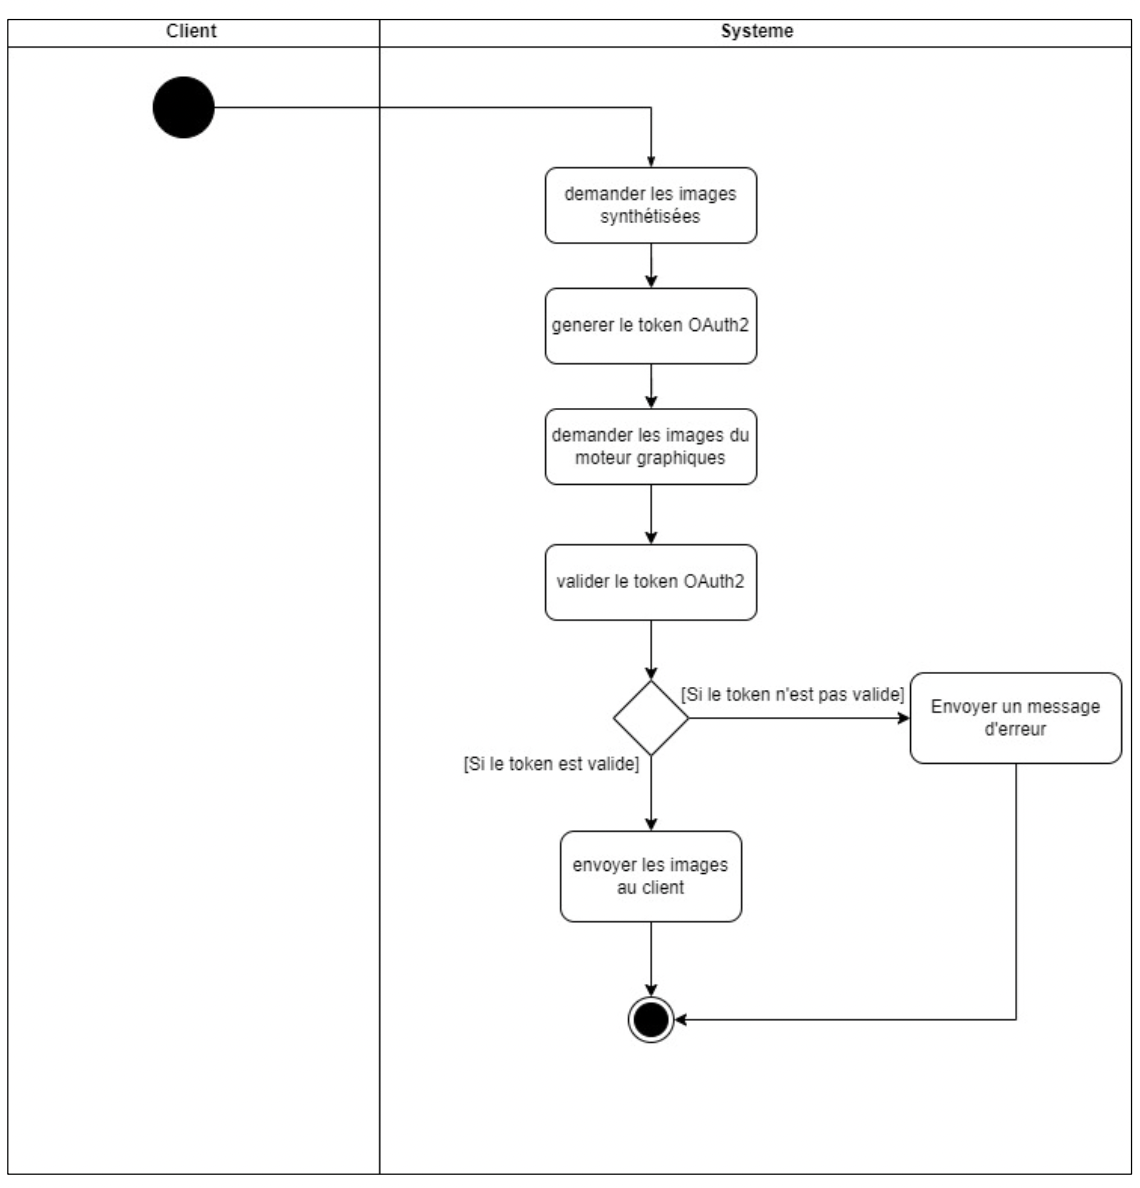
\includegraphics[width=1\textwidth,angle=00]{chapitres/chapitre4/figures/Act-Chap4.png}
% \caption{Diagramme\textcolor{white}{J}d’activité}
% \label{fig:digAct4}
% \end{figure}

% en demandant les images synthétisées,le systeme va generer une  clé d'authentification puis demander les images du moteur graphiques et les envoyer a la partie backend.Ensuite,le serveur backend procede a la validation de la cle d'authentification.Si la clé n'est pas valide,un message d'erreur est envoyé au client.Sinon les images synthétisées sont envoyées au client.

% \newpage
% \subsection{Diagramme\textcolor{white}{J}de\textcolor{white}{J}séquence\textcolor{white}{J}objet}
% \begin{figure}[!ht]\centering
% 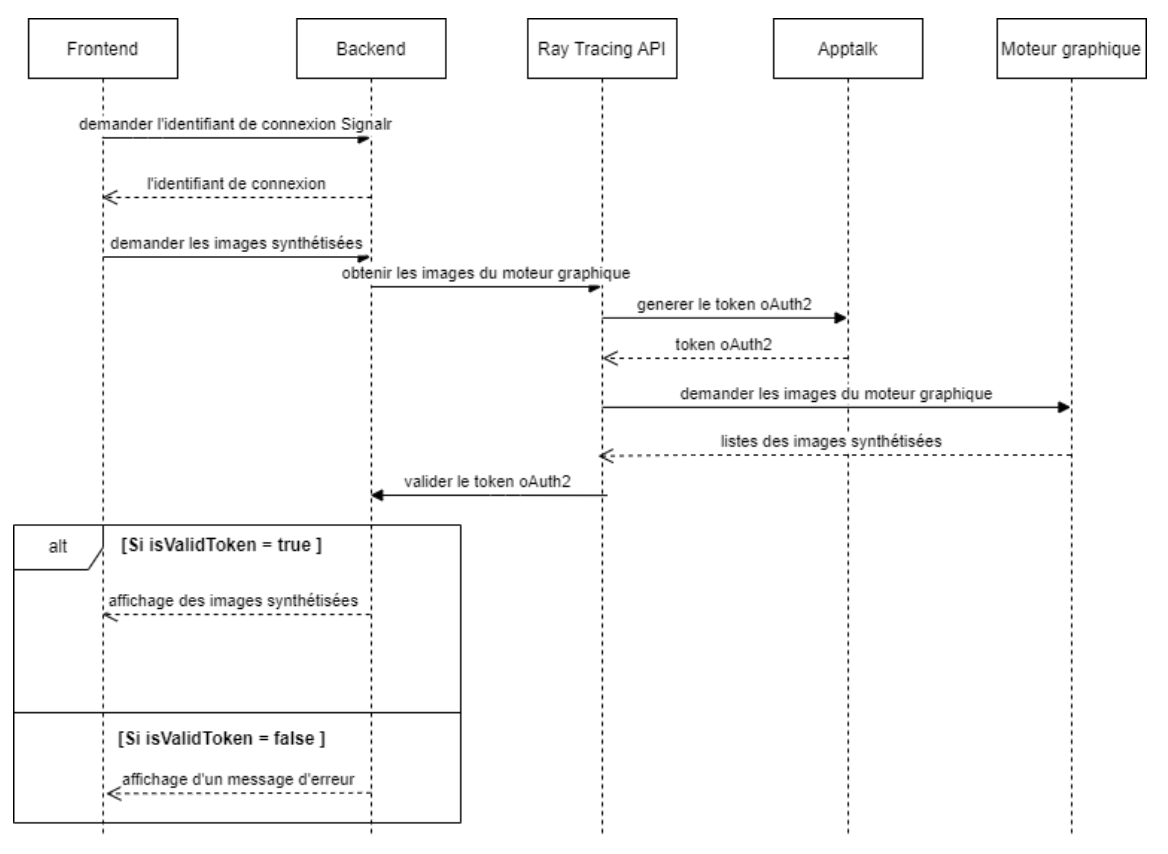
\includegraphics[width=0.8\textwidth,angle=00]{chapitres/chapitre4/figures/Seq-Chap4.png}
% \caption{Diagramme\textcolor{white}{J}de\textcolor{white}{J}séquence\textcolor{white}{J}objet
% }
% \label{fig:schemaSourcin}
% \end{figure}


% \subsection{Diagramme\textcolor{white}{J}de\textcolor{white}{J}séquence\textcolor{white}{J}de\textcolor{white}{J}la demande du jeton d’accès}
% \begin{figure}[!ht]\centering
% 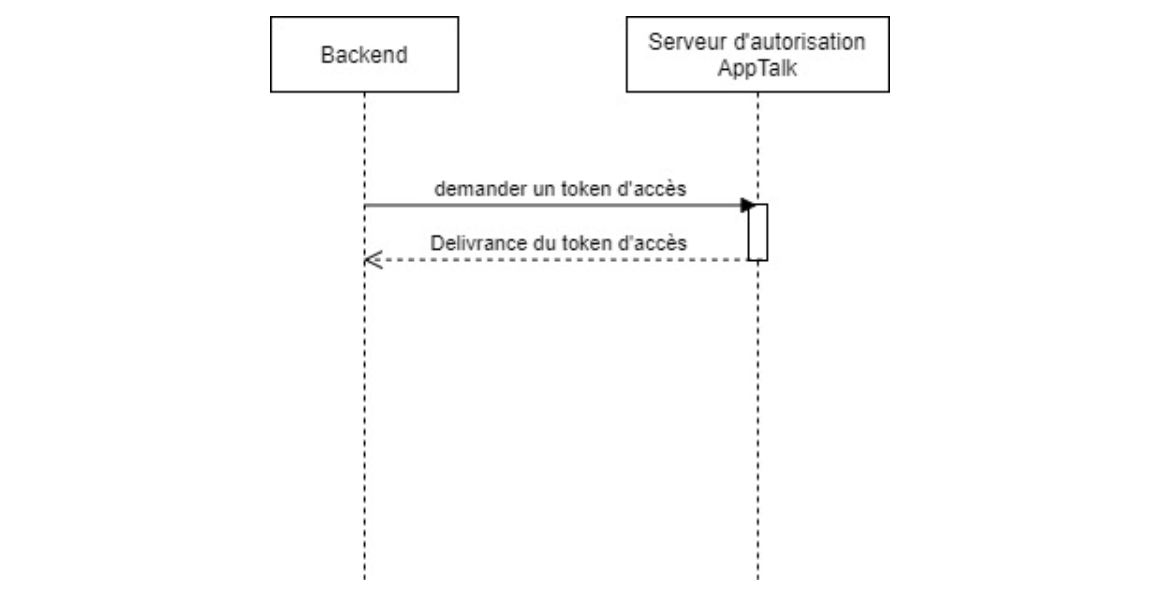
\includegraphics[width=0.9\textwidth,angle=00]{chapitres/chapitre4/figures/SeqDemande-Chap4.png}
% \caption{Diagramme de séquence de la demande du jeton d’accès}
% \label{fig:schemaSourcin}
% \end{figure}

% \newpage
% \subsection{Diagramme\textcolor{white}{J}de\textcolor{white}{J}classe\textcolor{white}{J}de\textcolor{white}{J}conception}
% \begin{figure}[!ht]\centering
% 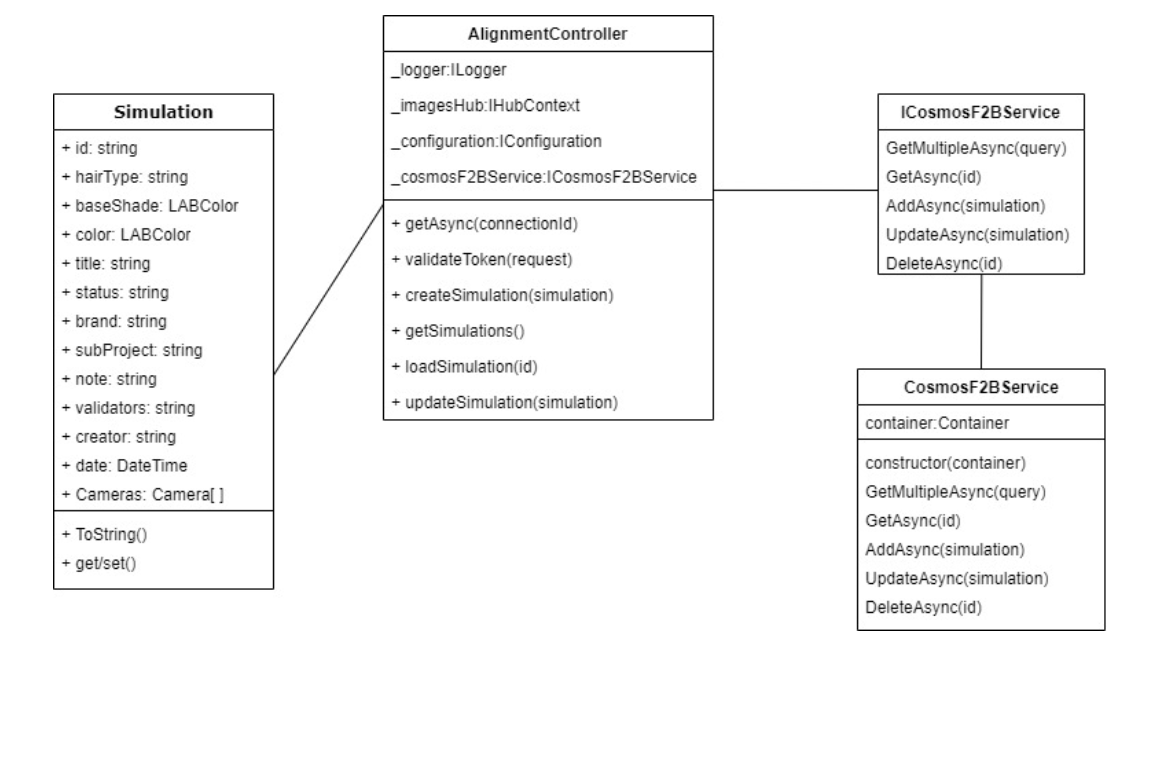
\includegraphics[width=0.9\textwidth,angle=00]{chapitres/chapitre4/figures/Class-Chap4.png}
% \caption{Diagramme\textcolor{white}{J}de\textcolor{white}{J}classe\textcolor{white}{J}de\textcolor{white}{J}conception}
% \label{fig:schemaSourcin}
% \end{figure}

% \section{Réalisation}

% \subsection{Technologies}
% \subsubsection*{Swagger[11]}
% À l’heure actuelle, Swagger est la meilleure solution pour documenter une API REST, car le système est capable de représenter presque tous les services Web et informations ayant trait à l’interface. La documentation évolue en même temps que le système et enregistre automatiquement les modifications. Swagger se montre particulièrement efficace pour parvenir à ce résultat parce qu’il consigne la documentation d’une API REST directement dans son code. Grace au fichier Swagger.json qui contient toutes les informations sur nos APIs, on peut générer le client HTTP pour accéder aux APIs dans le Frontend en utilisant le package Autorest.


% \newpage
% \subsubsection*{SignalR[12]}
% SignalR est une bibliothèque client/serveur pour Microsoft ASP.NET qui permet au code serveur d'envoyer des notifications asynchrones aux applications Web côté client. La bibliothèque comprend des composants JavaScript côté serveur et côté client. Il fournit également une API simple et de haut niveau pour effectuer des RPC de serveur à client (appeler des fonctions JavaScript dans le navigateur d'un client à partir du code .NET côté serveur) dans une application ASP.NET, ainsi que l'ajout de fonctions utiles pour la gestion des connexions tels que les événements de connexion/déconnexion et l’autorisation.



% \subsubsection*{Cosmos DB[13]}
% Azure Cosmos DB est une base de données NoSQL sans serveur, entièrement gérée, destinée aux applications hautes performances avec une vitesse garantie à n’importe quelle échelle avec un débit instantané et illimité, des lectures rapides et des écritures multirégion partout dans le monde.
Avec des kits de développement logiciel (SDK) pour les langages les plus courants, ainsi qu'une API Core (SQL) native, des API pour MongoDB, Cassandra et Gremlin



% \newpage
% \subsection{Mise en place de l’architecture cible}
% Après l’évolution de l’application OptixHair en un moteur graphique capable d’envoyer les images dans un bus de communication instantanée appelée websocket, on a développé la partie backend qui doit communiquer avec ce dernier.
% La partie backend est divisée en deux parties : 
% Une partie responsable a la communication avec le client intitulé Backend API et une partie qui communiquera avec le moteur graphique qui s’appelle SimulatorInterface API.
% La figure \ref{fig:cible} suivante représente l’architecture cible de ce sprint.

% \begin{figure}[!ht]\centering
% 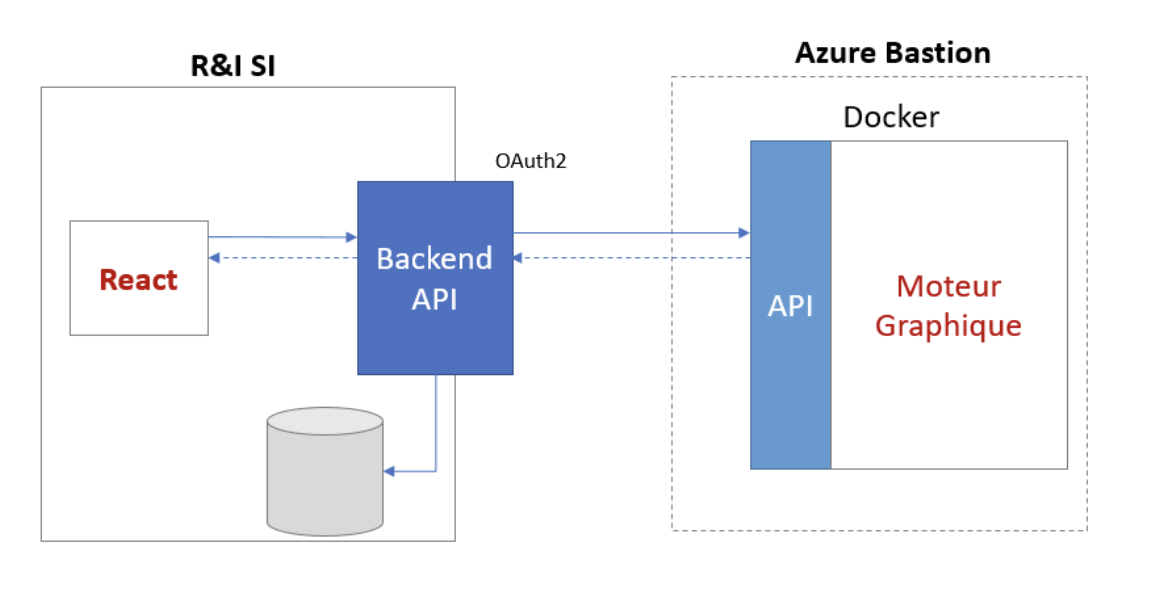
\includegraphics[width=0.9\textwidth]{chapitres/chapitre4/figures/ArchCible.png}
% \caption{L’architecture cible}
% \label{fig:cible}
% \end{figure}

% \subsection{Implémentation}
% \subsubsection{Développement de la partie Backend}
% 
Tout d’abord, on a développé une API fonctionnelle responsable de la communication entre le serveur Backend et le serveur de communication avec le moteur graphique. Cette API est exposée avec la méthode GET du protocole http sous le chemin « /Alignement/Get/ » et prend en paramètre l’identifiant de connexion du client qui demande les images synthétisées. 
% La figure suivante représente l’API de récupération des images.

% \begin{figure}[!ht]\centering
% 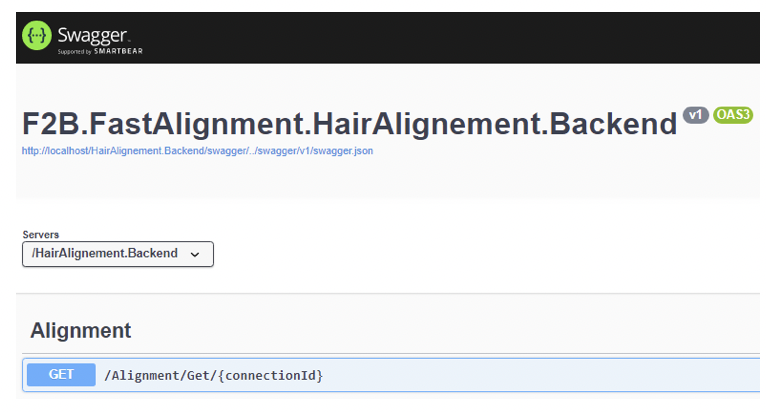
\includegraphics[width=0.8\textwidth]{chapitres/chapitre4/figures/AlignementGet.png}
% \caption{Récupération des images}
% \label{fig:git}
% \end{figure}

% Dans cette API, on a exécuté une requête au serveur « SimulatorInterface API » pour qu’il récupère les images synthétisées du moteur graphique et les renvoyés au serveur « Backend API » puis ce dernier va faire la redirection de ses images au client.

% \subsubsection{ Intégration du protocole d’autorisation OAuth2}
% Pour assurer l’authentification de cette communication, on a utilisé OAuth2 qui est un protocole d’autorisation largement utilisé par L’Oréal.
% La demande d'accès à une ressource protégée avec ce protocole se traduit par l'émission d'un jeton au client. Le jeton représente simplement une chaîne unique utilisée pour identifier le client et diverses informations utiles lors du processus d'autorisation. Ce dernier a une durée de validité limitée.
% Pour en obtenir un, le serveur « SimulatorInterface API » doit faire une requête au serveur d’autorisation AppTalk en précisant ces paramètres.

% \begin{figure}[!ht]\centering
% 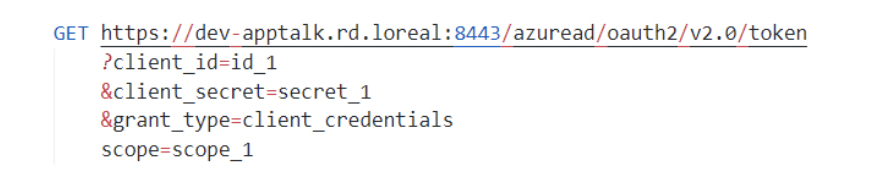
\includegraphics[width=0.8\textwidth]{chapitres/chapitre4/figures/Apptalk.png}
% \caption{Récupération des images}
% \label{fig:git}
% \end{figure}

% Si tout se passe bien, l’AppTalk renverrait une réponse contenant notre token d’accès.

% \begin{figure}[!ht]\centering
% 
\includegraphics[width=0.8\textwidth]{chapitres/chapitre4/figures/Apptalk-token.png}
% \caption{Récupération des images}
% \label{fig:git}
% \end{figure}

% \subsubsection{ Communication avec le moteur graphique}
% Après avoir récupérer le jeton d’accès, le serveur « SimulatorInterface API » va ouvrir une session de communication instantanée avec le moteur graphique pour récupérer les images synthétisées puis les renvoyées au serveur « Backend API » tout en spécifiant le jeton d’accès à l’entête. 

% La figure \ref{fig:comMoteur} suivante représente l’API de communication avec le moteur graphique.

% \begin{figure}[!ht]\centering
% 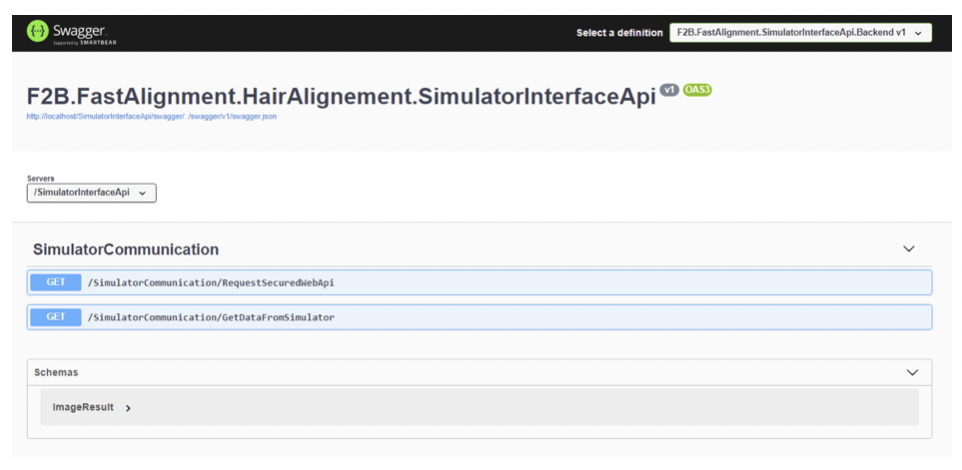
\includegraphics[width=0.7\textwidth]{chapitres/chapitre4/figures/SimuGet.png}
% \caption{Communication avec le moteur graphique}
% \label{fig:comMoteur}
% \end{figure}

% \subsubsection{ Validation du token et renvoie des images au client}
% Maintenant, le serveur « Backend API » doit tout d’abord vérifier la validité du token via l’API « validateToken », si le token est valide les images seront publiées au client le bus de communication SignalR. Dans le cas contraire une exception sera levée, l’envoie des images sera abandonné et le message d’erreur sera envoyé au client.
% La figure \ref{fig:vldToken} ci-dessous représente l’API de validation du token « validateToken ».

% \begin{figure}[!ht]\centering
% 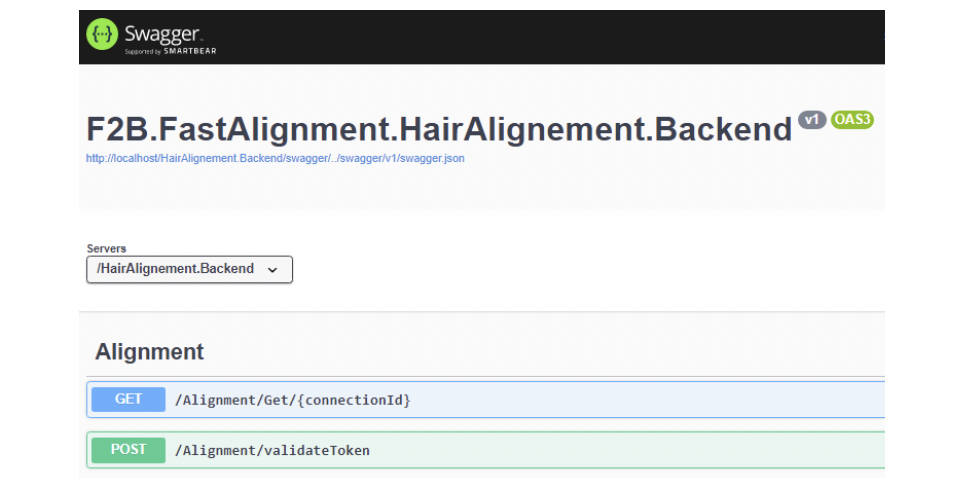
\includegraphics[width=0.7\textwidth]{chapitres/chapitre4/figures/AlignementPost.png}
% \caption{Api de validation du token}
% \label{fig:vldToken}
% \end{figure}

% \newpage
% \subsubsection{ Configuration de la base de données Cosmos DB}
% Pour le stockage des simulations, on a opté pour la base de données Cosmos DB qui est une base de données NoSQL distribué mondialement. Azure Cosmos DB est disponible dans toutes les régions Azure à travers le monde.
% Azure Cosmos DB organise les données dans une structure hiérarchique de bases de données, de conteneurs et d'éléments. Nous pouvons ajouter une base de données, des conteneurs et des éléments à partir du panneau Data Explorer de Cosmos DB.
% La figure \ref{fig:comCosmos} suivante présente le conteneur créé intitulé F2BContainer

% \begin{figure}[!ht]\centering
% 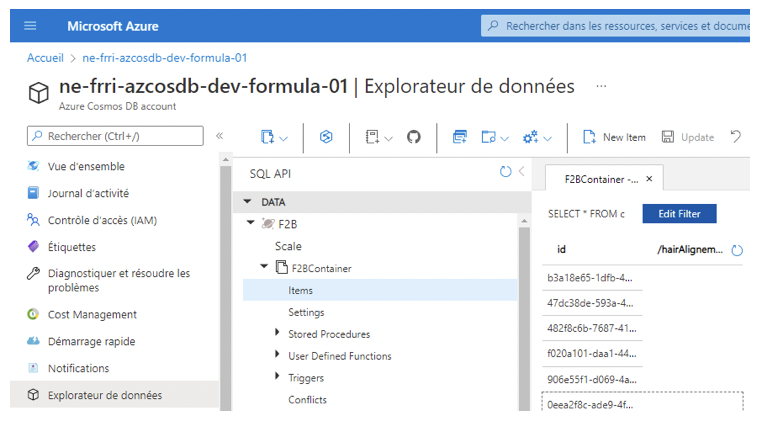
\includegraphics[width=0.8\textwidth]{chapitres/chapitre4/figures/Azure.png}
% \caption{Configuration de la base de données Cosmos DB}
% \label{fig:comCosmos}
% \end{figure}

% Maintenant que nous avons créé le conteneur, nous devons ajouter les packages NuGet nécessaires pour se connecter à Azure Cosmos DB.

% \begin{figure}[!ht]\centering
% 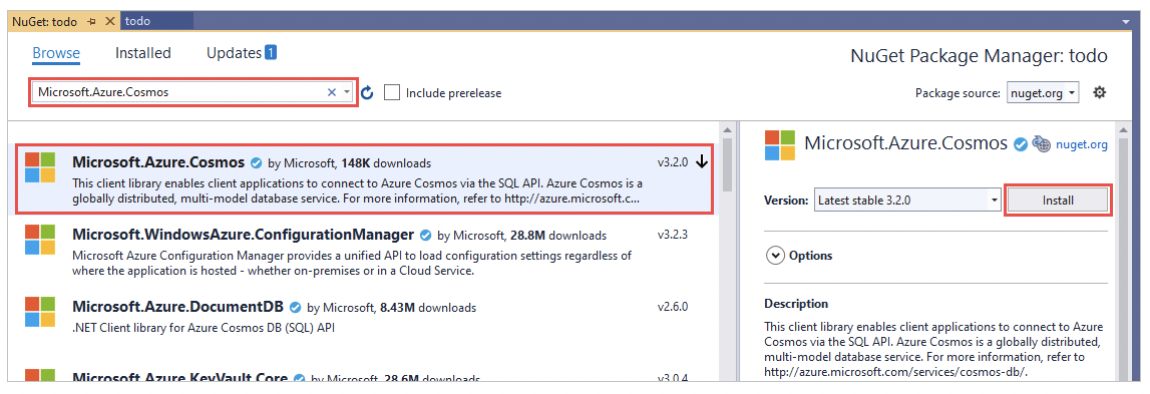
\includegraphics[width=0.8\textwidth]{chapitres/chapitre4/figures/CosmosDB.png}
% \caption{Configuration de la base de données Cosmos DB}
% \label{fig:git}
% \end{figure}

% \newpage
% Ensuite, nous avons ajouté une classe qui contient la logique pour se connecter et utiliser Azure Cosmos DB. Dans ce didacticiel, nous avons encapsulé cette logique dans une classe appelée « CosmosF2BService » et une interface appelée « ICosmosF2BService ». Ce service effectue des opérations CRUD. Il effectue également des opérations de lecture de flux telles que la liste des éléments incomplets, la création, la modification et la suppression d'éléments.

% Nous avons aussi ajouté la méthode « InitializeCosmosClientInstanceAsync » pour créer un client cosmos comme indiqué dans la figure ci-dessous. Cette fonction a besoin de ces paramètres pour pouvoir créer l’instance de connexion :
% \begin{figure}[!ht]\centering
% 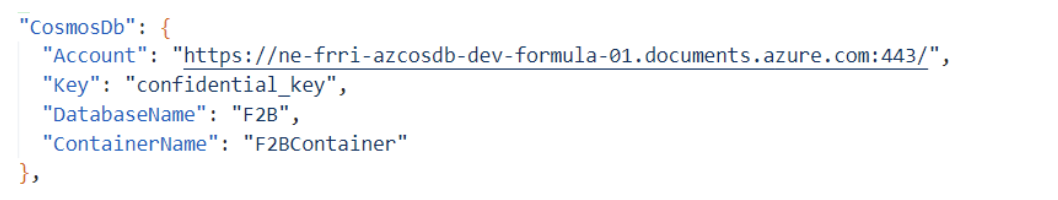
\includegraphics[width=0.8\textwidth]{chapitres/chapitre4/figures/CosmosDb-azure.png}
% \caption{InitializeCosmosClientInstanceAsync}
% \label{fig:git}
% \end{figure}

% \subsubsection{Créer l’API de sauvegarde des simulations}
% Pour utiliser les opérations CRUD qu’on a implémenté dans le service « CosmosF2BService », on a déclaré une variable de l’interface ce service en « readonly » pour faire l’injection de dépendance. Par la suite, on a créé quatre APIs fonctionnelles où on a fait l’appel des fonctions du service « CosmosF2BService »
% La figure \ref{fig:crud} ci-dessous présente les APIs des opérations CRUD

% \begin{figure}[!ht]\centering
% 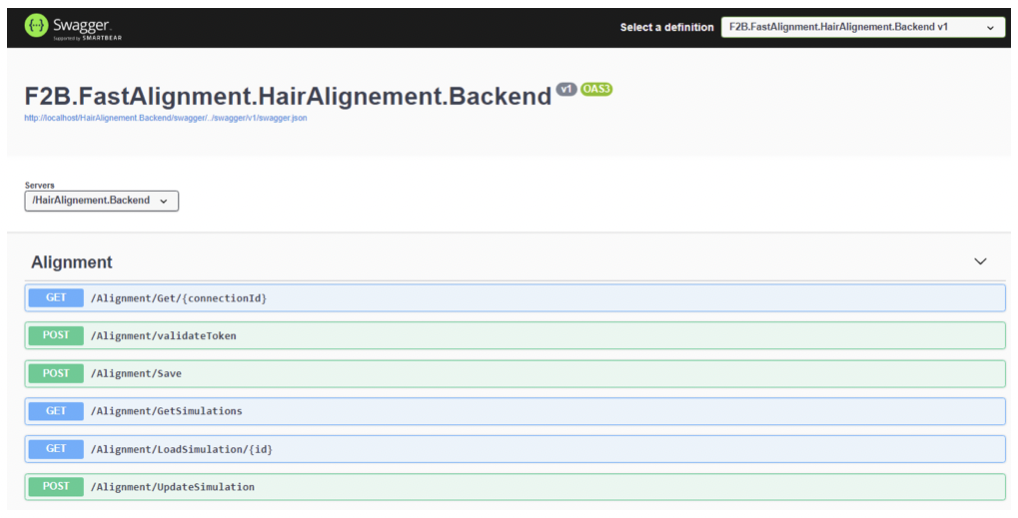
\includegraphics[width=0.8\textwidth]{chapitres/chapitre4/figures/crud.png}
% \caption{Les opérations CRUD}
% \label{fig:crud}
% \end{figure}


% \section*{Conclusion}
% Au cours de ce chapitre, nous avons réussi à développer la partie backend qui comporte la gestion des simulations et la mise en place du protocole d’authentification OAuth2. Dans le chapitre suivant, tout l’effort sera consacré pour développer la partie frontend puis l’intégration du projet dans la Formulation Center et enfin le déploiement de notre solution.



\graphicspath{{./assets/}}
\setcounter{mtc}{5}
\chapter{3rd Sprint: Resource provisioning  }
\fancyhead[R]{\ungaramond\small\textbf{Chapter V.  3rd Sprint: Resource provisioning  }}

\minitoc
\newpage
\section*{Introduction}



\section{Sprint Backlog}


\begin{longtable}[!ht]{|m{1.5cm}|m{3cm}|m{1.5cm}|m{9cm}|}
\hline
{\textbf{Epic ID}} & {\textbf{Epic}} & {\textbf{Story ID}} & {\textbf{Story}}\\
\hline
1  & Provisioning resources using IaC playbooks and HCP config files.  &  1.1	 & Preparing provider specific(ovh) terraform config. \\
\cline{3-4}
& & 1.2 & Preparing ansible playbook to initiate provisioning. \\
\cline{3-4}
& & 1.3	& Setting up IaC host machine.  \\
\cline{3-4}
& & 1.4	& Cloud provider account and project creation.  \\
\hline
\end{longtable}


\newpage

\section{UML design : class diagram for cloud infrastructure }


\section{“HCP config” diagram for cloud provisioning: }
The following figure illustrates the main resources declared in our terraform “HCP config”: 

\section{Component diagram of provisioned resources}

The cluster resources were deployed to three regions. Namely, GRA, BHS, SBG. In each region, four instances were created. One of which will join the control plane, two will have the worker compute role and the last will have a second block device in raw format and will join the data storage backend. Various buckets from the object store will be provisioned and will serve as backup storage backends and high speed data storage.  
\newpage


\section*{Conclusion}

\graphicspath{{./assets/}}
\setcounter{mtc}{5}
\chapter{4th Sprint }
\fancyhead[R]{\ungaramond\small\textbf{Chapter VI.  4th Sprint: Preliminary infrastructure setup   }}

\minitoc
\newpage
\section*{Introduction}



\graphicspath{{./chapitres/chapitre7/figures/}}
\setcounter{mtc}{7}
\chapter{Sprint Cinq: Expérimentation en Data Mining}
\minitoc
\newpage
\section*{Introduction}
Notre projet est en réalité un projet à long terme qui est divisé sur plusieurs parties. Ce que nous avons réalisé jusqu'ici est une première partie du projet.\newline
Concernant la suite du projet, c'est un nouveau mini projet pour mener une analyse avancée sur les transactions (prédiction,  classification, clustering ,etc).\newline
Dans ce chapitre nous allons mettre en place un petit exemple sous forme d'une expérimentation pour avoir une vision plus claire sur les prochaines étapes dans le futur.
\section{Sprint Backlog}
\subsection{Histoires \`a r\'ealiser}
Le tableau \ref{tab:sprint5backlog} d\'ecrit les histoires du backlog de ce sprint.

\begin{longtable}[!ht]{|l|l|c|}
\hline
{\textbf{Feature}} & {\textbf{Technical Story}} & {\textbf{Story Points}}\\
\hline
\multirow{2}{3cm}{\textbf{ Une formation Python et Flask}} & R\&D Python   & 3 \\
\cline{2-3}
& R\&D Flask et Flask-MongoEngine  & 5 \\
\cline{2-3}
&  R\&D algorithmes de data mining & 3 \\
\hline
\multirow{2}{4cm}{\textbf{Une formation Angular 7}} 
& Une recherche sur l'intégration Back/Front entre  & 3 \\
&Angular et Python &\\

\hline
\multirow{1}{4cm}{\textbf{Recherche et initiation}} & Initiation à la data science & 5  \\
\cline{2-3}
 &Initiation aux algorithmes de clustering  & 3\\
\cline{2-3}
 &Initiation à la visualisation clustering (dataviz) & 3\\
\hline
{\textbf{Test et développement }} & Expérimenter plusieurs algorithmes en & 3\\& utilisant Jupyter Notebook&\\
\cline{2-3}
 &Balancer les données avec Faker  & 3\\
 \cline{2-3}
 &Benchmark des algorithmes  & 3\\
\cline{2-3}
 &Analyser les données equilibrées avec Kmeans& 3\\
 \cline{2-3}
 &Déterminer un clustering général& 3\\
\cline{2-3}
 &Déterminer un clustering sur le type de&3 \\ & transaction et le montant& \\
\cline{2-3}
 &Déterminer un clustering sur les IDs des mandats & 3\\ &des transactionset le montant&\\
\cline{2-3}
 &Déterminer un clustering sur le pays de réception & 3\\ &  des transactions et le montant&\\
\cline{2-3}
 &Déterminer un clustering sur le pays d'envoi  & 3\\ & des transactions et le montant& \\
\cline{2-3}
 &Créer une API Restful pour assurer la génération  & 3\\ & des graphiques de visualisation & \\
\cline{2-3}
\hline
\multirow{1}{4cm}{\textbf{Consulter les Flux }} & Création du service Kmeans  & 5  \\
\cline{2-3}
 &Création du composant "flux" & 3\\
\hline

\caption{Liste des t\^aches du cinquième sprint}
\label{tab:sprint5backlog}
\end{longtable}

\subsection{Objectif du sprint}
L'objectif de ce sprint est d'implémenter la consultation des analyses des flux des transactions de tous les clients.
\section{Analyse}
\subsection{Description textuelle de "Consulter les flux"}
Nous allons commencer par analyser le cas d'utilisation "Consulter les flux".
Le tableau \ref{tab:choisirModeAuth} illustre la description textuelle de ce cas d'utilisation.
\begin{table}[!ht]
\begin{tabular}{|l|l|}
\hline
\rowcolor{lightgray}{\textbf{Titre}} & Consulter les flux\\
\hline
\rowcolor{lightgray}{\textbf{Acteur}} & Admin \\
\hline
{\textbf{But}} & L'admin peut consulter les statistique generale\\
\hline
{\textbf{Pr\'e-condition}} & L'admin doit s'authentifier et acc\'eder \`a \\ & le  page flux \\
\hline
{\textbf{Post-condition}} & Consulter les statiqtique\\
\hline
\multirow{2}{2cm}{\textbf{Sc\'enario nominal}} & 1. L'utilisateur se connecte \`a l'application par son login et mot de passe. \\
& 2. L'utilisateur clique sur le bouton \textbf{"Flux"}\\& du menu \`a gauche.   \\
& 3. Le syst\`eme affiche le detaille de l'interface .\\
\hline
\end{tabular}
\caption{Description textuelle du cas d'utilisation "Consulter les flux"}
\label{tab:choisirModeAuth}
\end{table}
\section{ Etapes de réalisation}
\begin{enumerate}
    \item
En effet, nous nous proposons d'effectuer la méthode de clustering sur les données des transactions dont nous disposons, et ce pour pouvoir mieux comprendre les comportements transactionnels des clients et créer des regroupement de transactions.
    \item
Puisque nous allons implémenter l'analyse des données pour la première fois pour notre application, et puisque nos données ne sont pas étiquetées, alors il n'est pas possible d'utiliser des algorithmes supervisés (qui affectent un score d'adéquation au résultat) donc nous allons appliquer un regroupement (Clustering) non supervisé.
\item Aprés une petite recherche, nous avons trouvé plusieurs algorithmes non supervisés ; et les deux algorithmes les plus pratiqués et les plus adaptés dans notre cas sont Random Forest et K-means.
\item Nous avons utilisé l'outil Jupyter Notebook pour tester plusieurs exemples de ces algorithmes mais nous avons trouvé un problème d'équilibrage dans nos données. Par conséquent, nous avons fait recours à la bibliothèque Faker pour ajouter des jeux de donnés dans notre base puis nous avons retesté les algorithmes sur ces nouvelles données équilibrées.
\item \textbf{Choix entre l'algorithme Random Forest et l'algorithme K-means}
\newline
\underline {Les Avantages de l'algorithme K-means:}
\begin{itemize}
    \item Simple:
Il est facile d’implémenter k-means et d’identifier des groupes de données inconnus à partir d’ensembles de données complexes. Les résultats sont présentés de manière rapide.
\item Flexible:
L’algorithme K-means s’adapte aux divers changements de vos données. En cas de souci, l’ajustement du segment de cluster permettra d’apporter rapidement des modifications nécessaires à l’algorithme.
\item Efficace:
L’algorithme utilisé permet de partitionner les gros de datasets. Son efficacité est fonction de la forme des clusters. Les K-Means fonctionnent bien dans les clusters hyper-sphériques.
\item Complexité temporelle:
La segmentation en K-Means est linéaire en nombre d’objets de données, ce qui augmente le temps d’exécution. Il ne faut pas plus de temps pour classer des caractéristiques similaires dans des données telles que des algorithmes hiérarchiques.


\item Convient aux gros data sets:
K-means convient à un grand nombre d’ensembles de données et est calculé beaucoup plus rapidement que le plus petit. Il peut également produire des clusters plus élevées.
\item Facile à interpréter:
Les résultats sont très faciles à interpréter. K-Means génère des descriptions de cluster sous une forme minimisée pour maximiser la compréhension des données.
\item Faible coût de calcul:
Comparée à l’utilisation d’autres méthodes de classification, une technique de classification k-means est rapide et efficace en termes de coût de calcul, en effet sa complexité est O (K * n * d).
\item Clusters sphériques:
Ce mode de regroupement fonctionne très bien lorsqu’il s’agit de clusters sphériques.
\end{itemize}
\underline {Les Avantages de l'algorithme Random Forest:}
\begin{itemize}
    \item L'arbre de décision est devenu une méthode
très prisée au vu de la rapidité de ses temps de calcul, de
sa capacité à gérer tous types de variables et à sélectionner
les plus pertinentes, ainsi que la lisibilité et la facilité
d'interprétation des résultats
\end{itemize}
\underline {Les inconvénients de l'algorithme K-means:}
\begin{itemize}
    \item Ensemble non optimal de clusters:
K-means ne permet pas de développer un ensemble optimal de clusters et vous devez choisir les clusters avant pour des résultats effectifs.
\item Manque de cohérence:
Le clustering K-means donne des résultats variables sur différentes exécutions d’un algorithme. Un choix aléatoire de modèles de clusters produit différents résultats, ce qui entraîne une incohérence.


\item Effet uniforme:
Il produit un cluster de taille uniforme même lorsque les données d’entrée ont des tailles différentes.
\item Spécifiez les valeurs K:
pour que la classification par K-moyennes soit efficace, vous devez spécifier le nombre de clusters (K) au début de l’algorithme.
\end{itemize}
\underline {Les inconvénients de l'algorithme Random Forest:}
\begin{itemize}
    \item L'inconvénient principal des arbres de
décision est que la classification dépend fortement de
l'ordre des variables choisies ce qui peut nuire au pouvoir
prédictif du modèle. Cette limite peut être rectifiée par des
techniques de boosting ou bagging.


\end{itemize}
Nous allons utiliser dans ce qui suit l'algorithme K-Means.

\end{enumerate}
\section{Conception}
\subsubsection{Modélisation dynamique : Diagramme de s\'equence}
Le diagramme de s\'equence du cas d'utilisation "Consulter les flux" est illustré par la figure \ref{fig:SequenceDiagramFlux}.
\newpage
\begin{figure}[!htbp]\centering
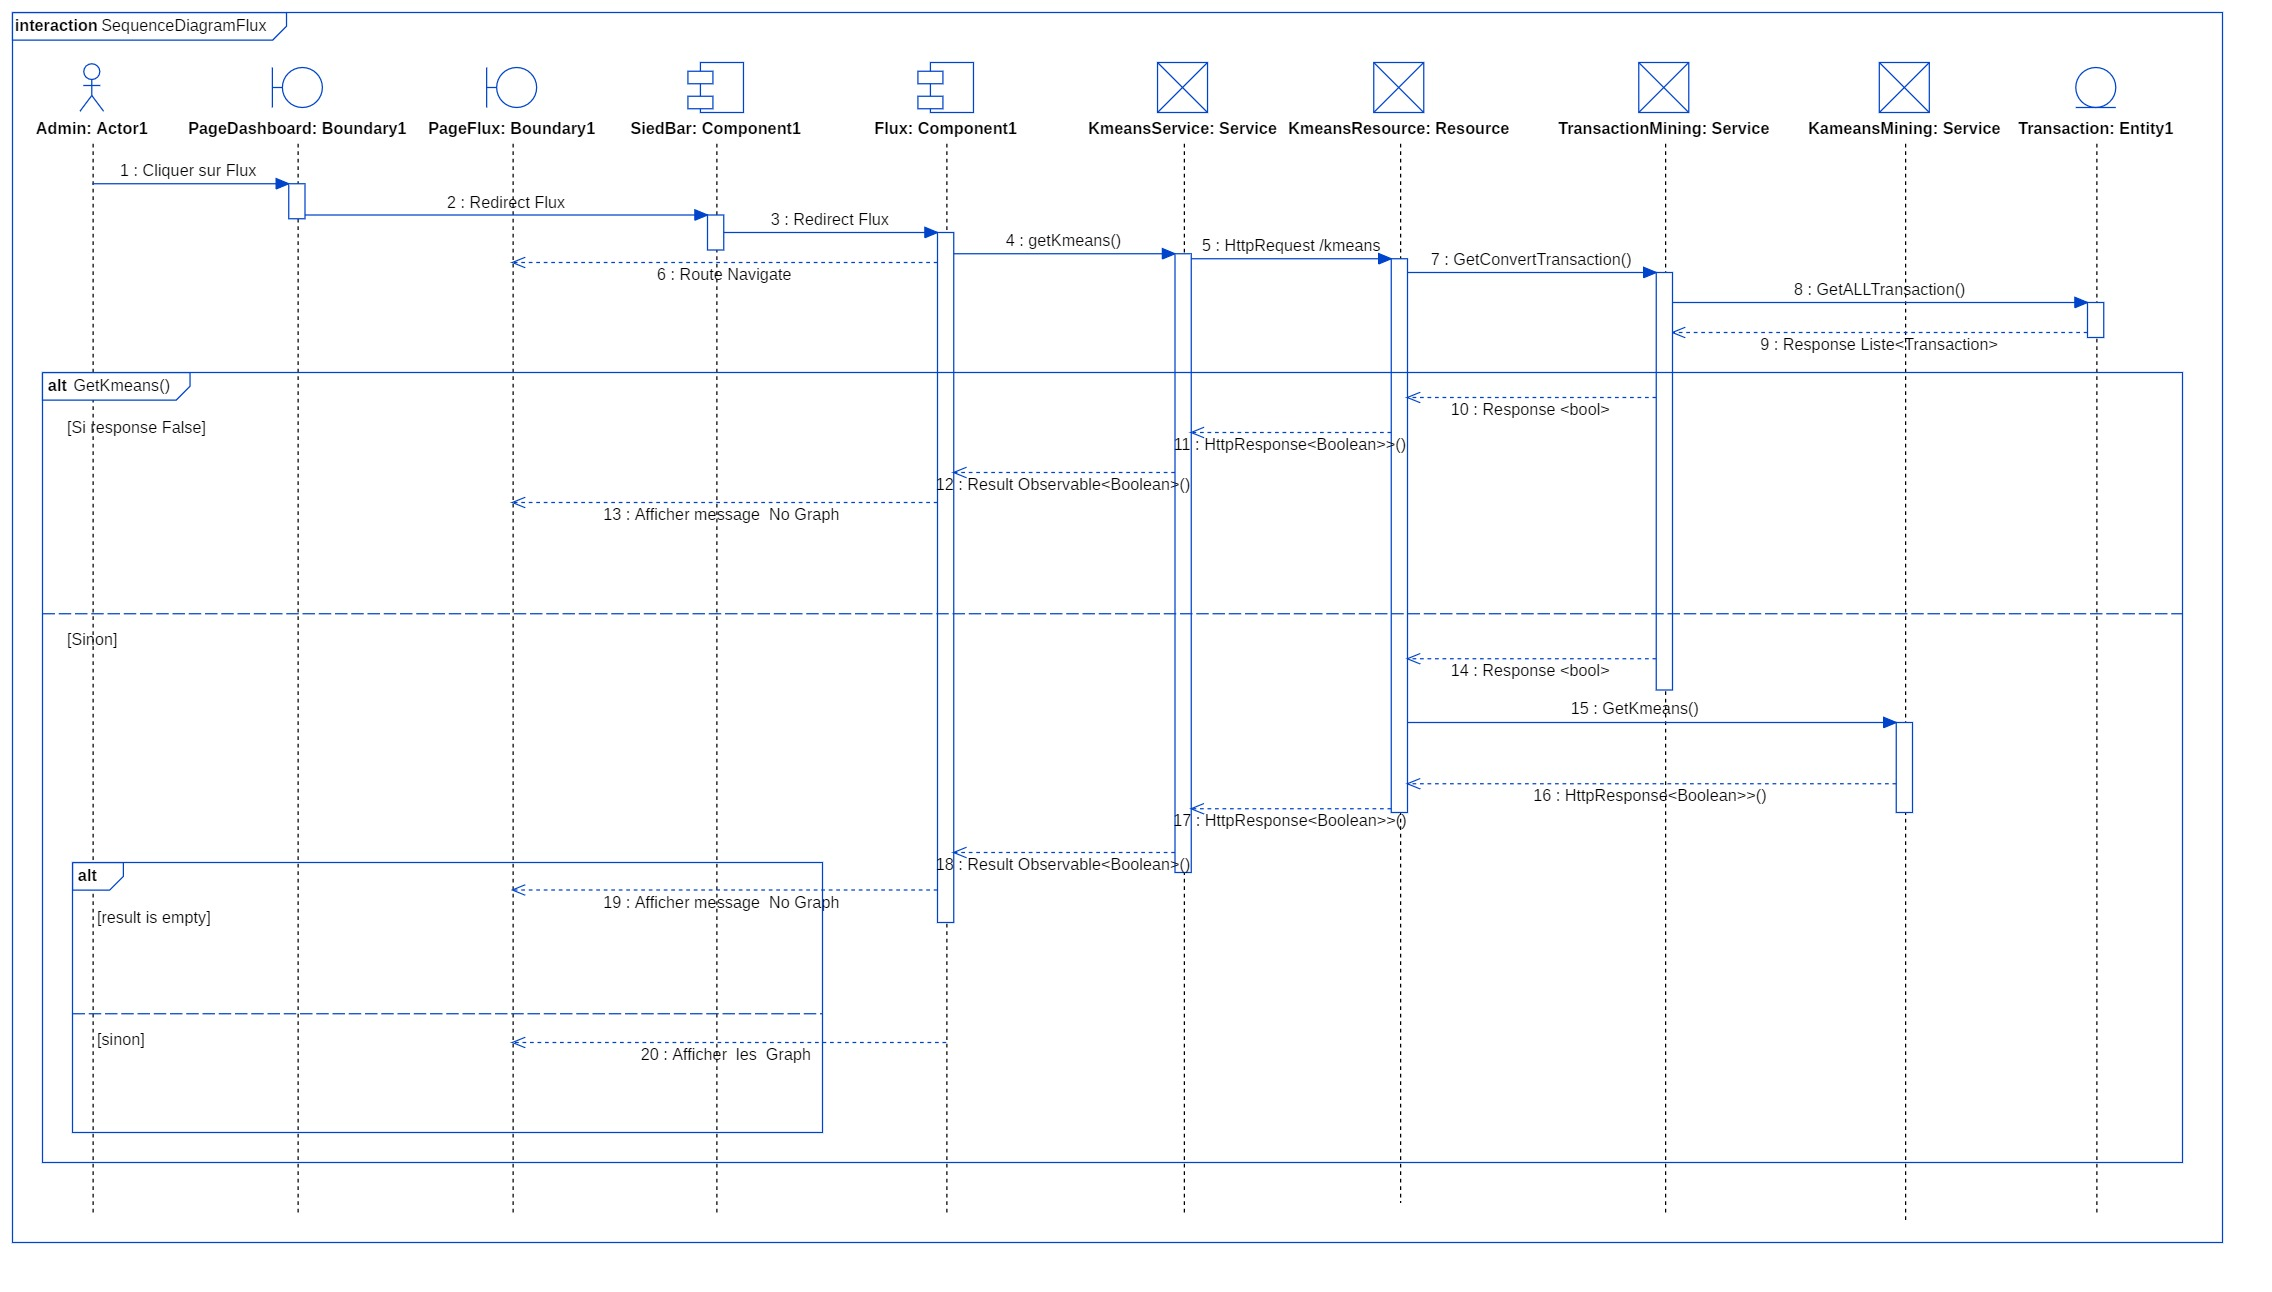
\includegraphics[width=1.4\columnwidth,angle=90]{chapitres/chapitre7/figures/SequenceDiagramFlux.jpg}
\caption{Diagramme de séquence du cas d'utilisation "Consulter les fluxe"}
\label{fig:SequenceDiagramFlux}
\end{figure}
\section{Réalisation}
L'interface illustrée dans la figure \ref{fig:flux1} permet d'afficher la premières partie
 des graphiques qui présentent le résultat des analyses de flux. 

\begin{figure}[!ht]\centering
\fbox{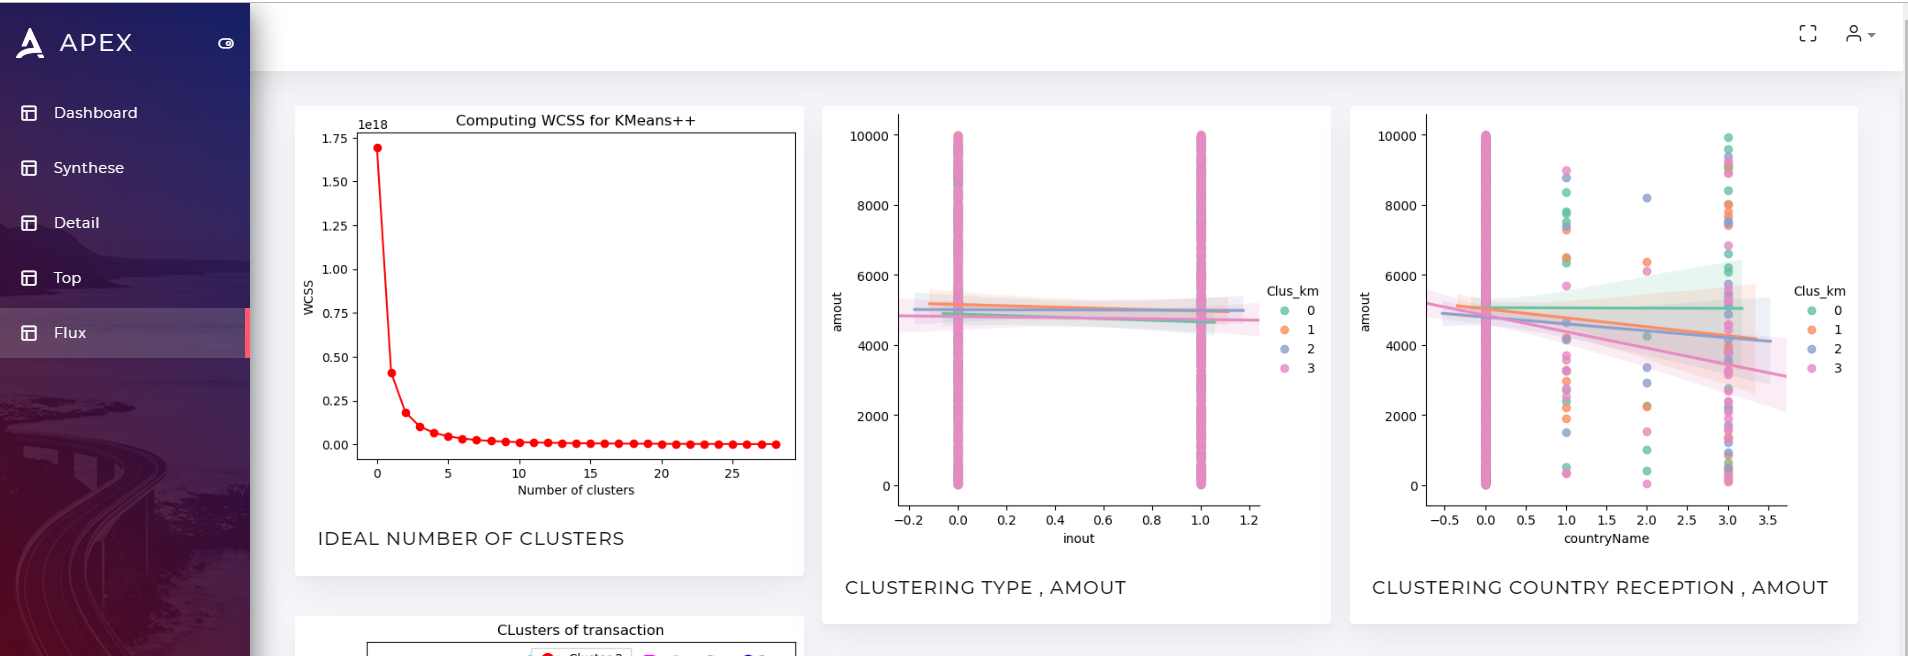
\includegraphics[width=1\textwidth]{chapitres/chapitre7/figures/flux1.PNG}}
\caption{Interface consulter les flux}
\label{fig:flux1}
\end{figure} 
L'interface illustrée dans la figures \ref{fig:flux1} permet d'afficher la deuxième partie   
 des graphiques qui présentent le résultat des analyses de flux.  
\begin{figure}[!ht]\centering
\fbox{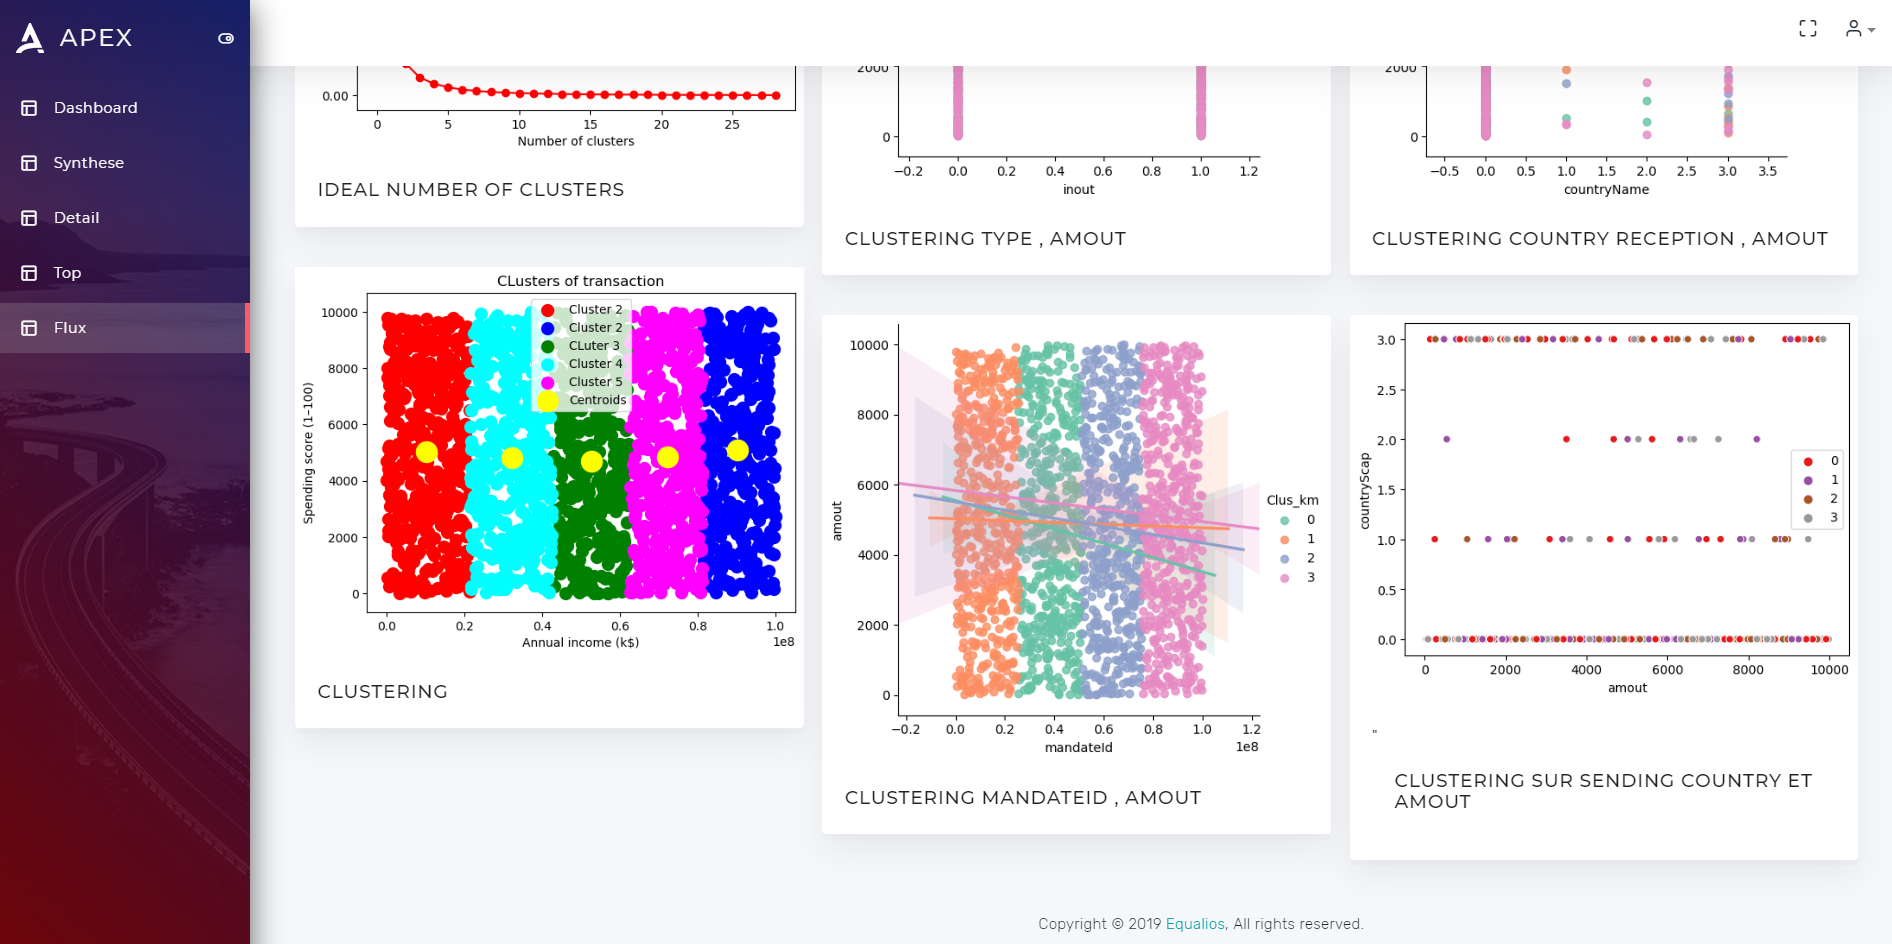
\includegraphics[width=1\textwidth]{chapitres/chapitre7/figures/flux2.PNG}}
\caption{Interface consulter les flux}
\label{fig:flux2}
\end{figure} 
\section{Environnement de travail}
Dans ce chapitre nous avons découvert une autre vision, d'autres technologies, langages et logiciels.
\subsection{Environnement logiciel}
\subsubsection*{PyCharm }
PyCharm est un environnement de développement intégré utilisé pour programmer en Python,  d\'evelopp\'e par l'entreprise JetBrains .
\begin{figure}[!ht]\centering

\includegraphics[width=0.2\textwidth]{chapitres/chapitre7/figures/pycharme.png}
\caption{Pycharm logo}
\label{fig:pycharme}
\end{figure}
\subsubsection*{Jupyter Notebook }
Jupyter Notebook est une application web utilisée pour programmer dans plus de 40 langages de programmation, dont Python, Julia, Ruby, R, ou encore Scala2. Jupyter est une évolution du projet IPython. Jupyter permet de réaliser des calepins ou notebooks, c'est-à-dire des programmes contenant à la fois du texte en markdown et du code en Julia, Python, R... Ces notebooks sont utilisés en science des données pour explorer et analyser des données.
\begin{figure}[!ht]\centering

\includegraphics[width=0.2\textwidth]{chapitres/chapitre7/figures/Jupyter.png}
\caption{Jupyter logo}
\label{fig:Jupyter}
\end{figure}
\subsection{Argumentation des choix techniques}
\subsubsection*{Python}
Python est un langage de programmation interprété, orienté objet et de haut niveau avec une sémantique dynamique. Ses structures de données intégrées de haut niveau, combinées à un typage dynamique et à une liaison dynamique, le rendent très attrayant pour le développement rapide d'applications, ainsi que pour son utilisation en tant que langage de script ou de collage pour connecter des composants existants. La syntaxe simple et facile à apprendre de Python met l'accent sur la lisibilité et réduit donc le coût de la maintenance du programme. Python prend en charge les modules et les packages, ce qui encourage la modularité du programme et la réutilisation du code. L'interpréteur Python et la vaste bibliothèque standard sont disponibles gratuitement sous forme binaire ou source pour toutes les principales plates-formes et peuvent être distribués librement.
\begin{figure}[!ht]\centering

\includegraphics[width=0.4\textwidth]{chapitres/chapitrex/figures/python.png}
\caption{Python logo }
\label{fig:python}
\end{figure}
\subsubsection*{Flask}
Flask est un micro-framework web écrit en Python. Il s’agit d’un microframework car il ne nécessite ni outils ni bibliothèques particuliers. ... Cependant, Flask prend en charge des extensions pouvant ajouter des fonctionnalités d'application comme si elles étaient implémentées dans Flask même.
\begin{figure}[!ht]\centering
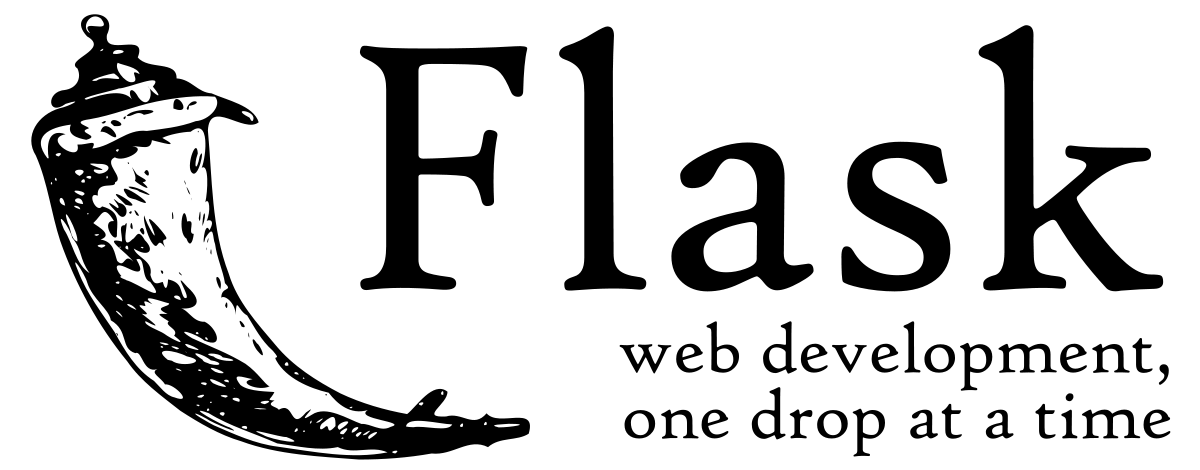
\includegraphics[width=0.4\textwidth]{chapitres/chapitre7/figures/flask.png}
\caption{Flask logo }
\label{fig:flask}
\end{figure}


\subsubsection*{Clustering K-means}

Le clustering K-means est l'un des algorithmes d'apprentissage automatique non supervisés les plus simples et les plus répandus.
En règle générale, les algorithmes non supervisés font des inférences à partir d'ensembles de données en utilisant uniquement des vecteurs d'entrée sans faire référence à des résultats connus ou étiquetés.
AndreyBu, qui a plus de 5 ans d'expérience en apprentissage automatique et enseigne actuellement ses compétences aux gens, déclare que «l'objectif de K-means est simple: regrouper des points de données similaires et découvrir les modèles sous-jacents. Pour atteindre cet objectif, K-means cherche un nombre fixe (k) de grappes dans un jeu de données. "
\begin{figure}[!ht]\centering
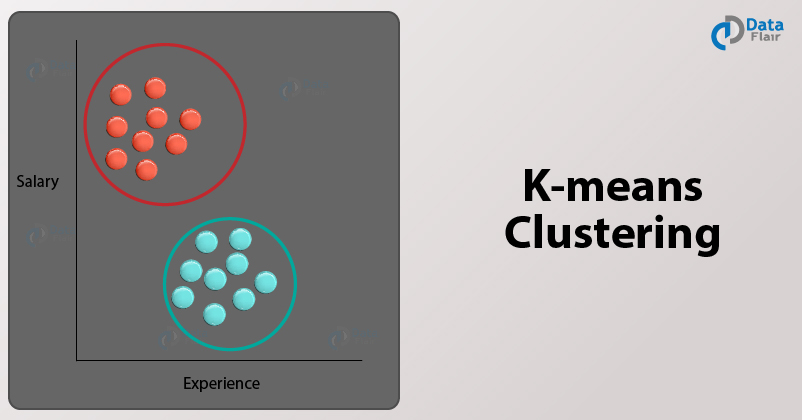
\includegraphics[width=0.4\textwidth]{chapitres/chapitre7/figures/KmeansClustering.jpg}
\caption{KmeansClustering }
\label{fig:KmeansClustering}
\end{figure}
\subsubsection*{Matplotlib}
Matplotlib a vu le jour pour permettre de générer directement des graphiques à partir de Python. Au fil des années, Matplotlib est devenu une librairie puissante, compatible avec beaucoup de plateformes, et capable de générer des graphiques dans beaucoup de formats différents.
\begin{figure}[!ht]\centering
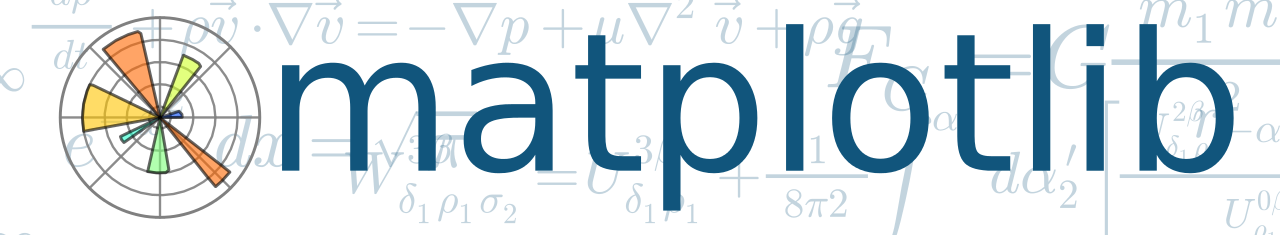
\includegraphics[width=0.4\textwidth]{chapitres/chapitre7/figures/Matplotlib.png}
\caption{Matplotlib logo }
\label{fig:matplotlib}
\end{figure}
\subsubsection*{Pandas}
Pandas est une bibliothèque écrite pour le langage de programmation Python permettant la manipulation et l'analyse des données. Elle propose en particulier des structures de données et des opérations de manipulation de tableaux numériques et de séries temporelles. Pandas est un logiciel libre sous licence BSD.
\newpage
\begin{figure}[!ht]\centering

\includegraphics[width=0.4\textwidth]{chapitres/chapitre7/figures/pandas.jpg}
\caption{Pandas logo }
\label{fig:pandas}
\end{figure}
\subsubsection*{Faker}
faker fait partie de ses libs que j’ai toujours voulu écrire sans jamais prendre le temps de le faire. Comme arrow par exemple. Et puis un jour quelqu’un le fait, et je suis à la fois soulagé de ne pas avoir tenté de le faire (au risque de ne pas réussir aussi bien) et un peu déçu d’être passé à côté de la bonne idée.

Le principe de la lib est très simple : générer des données bidons. Noms, numéros de téléphone, adresses physiques ou email… C’est utile pour tout un tas de choses :
\begin{enumerate}[label=$\bullet$]

    \item Faire des tests, évidement.
\item Créer des bots, des crawlers et tout autre programme qui doit se faire passer pour un utilisateur.
\item Remplir une base de données vide en attendant que les utilisateurs réels remplissent le site. Cela évite le sentiment d’arriver sur un service désert. Tous les sites de rencontre font ça.
\item Générer un contexte artificiel, par exemple pour un jeu vidéo.
\end{enumerate}
\begin{figure}[!ht]\centering

\includegraphics[width=0.4\textwidth]{chapitres/chapitre7/figures/faker.png}
\caption{Faker logo }
\label{fig:faker}
\end{figure}
\section*{Conclusion}
Lors de ce chapitre, nous avons r\'ealis\'e une petite expérimentation analysant des flux de transactions afin d'avoir une vision globale de notre base de données et de nous préparer pour passer à d'autres missions.

\graphicspath{{./chapitres/chapitre8/figures/}}
\setcounter{mtc}{8}
\chapter{Sprint Six : Déploiement de l'application}
\minitoc
\newpage
\section*{Introduction}
Au sixième chapitre nous avions parlé du l'architec déploiement de l'application et de la configuration technologique.
Il étale par la même occasion la procédure du déploiement de l'application et la configuration technologique.

\section{Conception architecturale}
\subsection{Architecture g\'en\'erale}
Cette section est consacr\'ee \`a d\'eterminer et d\'elimiter la vision globale de l'architecture technique \`a mettre en \oe uvre. 

En effet, d'apr\`es les exigences fonctionnelles \'etudi\'ees, notre solution fera n\'ecessairement l'objet d'une application Web. Le support du Web s'av\`ere le plus ad\'equat pour les applications complexes d\'elivr\'ees \`a partir d'une infrastructure centralis\'ee pour des clients l\'egers. 

Notre application Web repose sur une architecture trois-tiers (Client l\'eger-Serveur d'application-Serveur de base de donn\'ees).

L'architecture globale est introduite par la figure \ref{fig:architecture} qui montre explicitement le principe de la s\'eparation des trois niveaux suivants :
\begin{itemize}
\item La pr\'esentation des donn\'ees : Il s'agit d'un client l\'eger qui \'etablit une communication avec un serveur d'application et lance une requ\^ete afin d'obtenir un r\'esultat tangible souhait\'e.
\item La Logique m\'etier (le traitement m\'etier des donn\'ees) : c'est le niveau qui prend en charge la mise en \oe uvre de l'ensemble des r\`egles de gestion et de la logique applicative. Un serveur d'application s'occupe de traiter les requ\^etes reçues par le client et de lui renvoyer une r\'eponse.
\item Les donn\'ees : ce troisi\`eme et dernier niveau concerne les donn\'ees persistantes qui sont destin\'ees \`a \^etre acc\'ed\'ees et utilis\'ees par notre application. Ces donn\'ees sont conserv\'ees sur la dur\'ee, voire de mani\`ere d\'efinitive. Le serveur de base de donn\'ees reçoit des requ\^etes de la part du serveur d'application et consulte la base de donn\'ees derri\`ere pour restituer les donn\'ees demand\'ees (ou bien effectuer toute autre op\'eration de manipulation de donn\'ees).
\end{itemize}
\begin{figure}[!ht]\centering
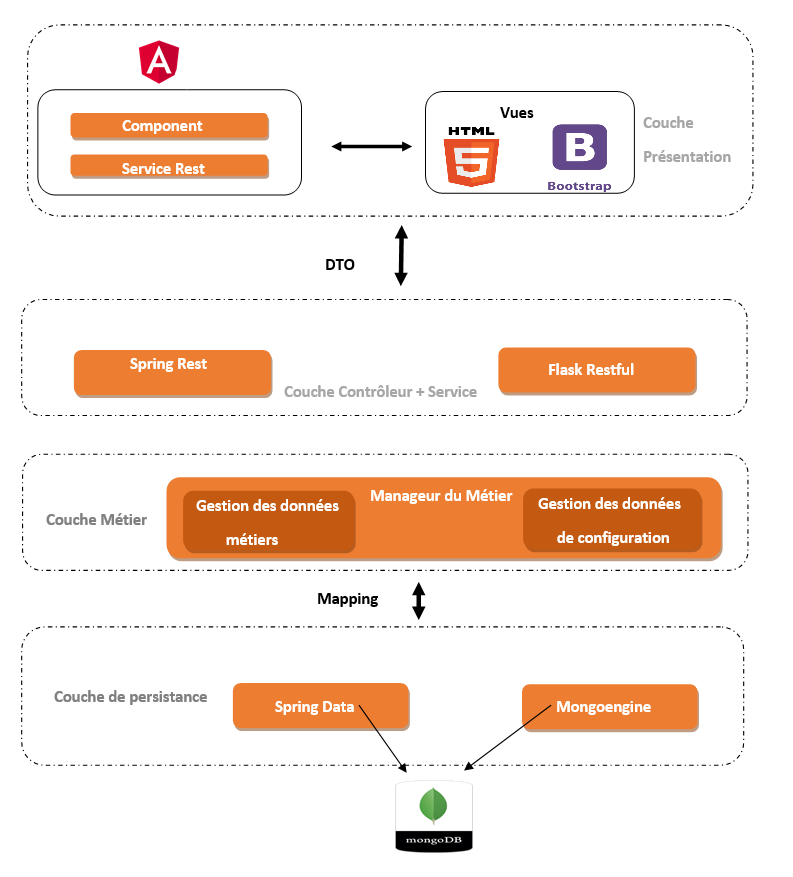
\includegraphics[scale=0.8]{architecture}
\caption{Architecture globale}
\label{fig:architecture}
\end{figure}

\subsection{Architecture d\'etaill\'ee}

L'architecture de notre application se caract\'erise par les couches suivantes :
\subsubsection*{La couche Pr\'esentation (Couche Web)}
Cette couche s'occupe des interactions directes avec l'utilisateur final (le client l\'eger) ; nous y trouvons des \'el\'ements tels que : des contr\^oleurs, des gestionnaires d'utilisateurs, des groupes, des r\^oles, des fonctionnalit\'es, et dans
notre cas la sous-couche DTO (Data Transfer Object).
\paragraph{La couche DTO}
Cette couche sert \`a d\'eplacer les donn\'ees vers et à partir de la couche de pr\'esentation. Id\'ealement, ceci se fait \`a travers la cr\'eation d'objets qui sont utilis\'es pour transmettre des donn\'ees \`a partir de la couche de pr\'esentation \`a la couche Services, et inversement. Un objet de transfert de donn\'ees (DTO) d\'etient toutes les donn\'ees qui sont nécessaires pour l'appel distant d'une des couches Présentation et Services.

\subsubsection*{La couche Logique M\'etier}
Cette couche constitue le c\oe ur du m\'etier ; c'est \`a dire le traitement (aspect fonctionnel et op\'erationnel transform\'e \`a partir de la sp\'ecification des besoins) derri\`ere l'application. Elle renferme elle-même plusieurs sous-couches. Les
contr\^oleurs de la couche Pr\'esentation acc\`edent \`a cette couche (plus pr\'ecis\'ement \`a travers la sous-couche "Services").
\paragraph{La couche contrôlleurs}
Cette couche permet d'exposer, comme son nom l'indique, des services exploitables par des tierces parties (Couche Pr\'esentation). C'est l'impl\'ementation des r\'egles de gestion m\'etier.
\paragraph{La couche DAO/Acc\`es aux Donn\'ees}
Les objets d'acc\`es aux donn\'ees (DAOs) se comportent r\'eellement comme une couche d'abstraction des donn\'ees (physiques)
pour les couches Entit\'es et Services. Ils se chargent de la manipulation des entit\'es en requ\^etant directement le serveur de base de donn\'ees et s\'eparent les acc\`es donn\'ees requis par l'application, en termes d'objets m\'etier sp\'ecifiques et de types de donn\'ees.
\paragraph{La couche Entit\'es}
Celle-ci regroupe toutes les entit\'es et les classes de mapping correspondant aux donn\'ees persistantes (tables) de la base de donn\'ees. Elle n'est accessible qu'au niveau de la couche Services et la couche DAO. Cette isolation permet d'affaiblir \'enorm\'ment le couplage entre ces objets et les \'el\'ements de la couche Pr\'esentation.
\subsubsection*{La Couche Infrastructure}

\paragraph{La couche Configuration}
Celle-ci permet de d\'efinir des configurations de certains \'el\'ements configurables de l'application (la couche web, la couche s\'ecurit\'e et la couche DAO par exemple) \`a des fins diff\'erentes. Elle contient des classes de configuration
ainsi que des fichiers de propri\'et\'es.

\section {Diagramme de déploiement}
La figure \ref{fig:DeploymentDiagram1} présente le diagramme de déploiement de notre solution.  

\begin{figure}[!ht]\centering
\fbox{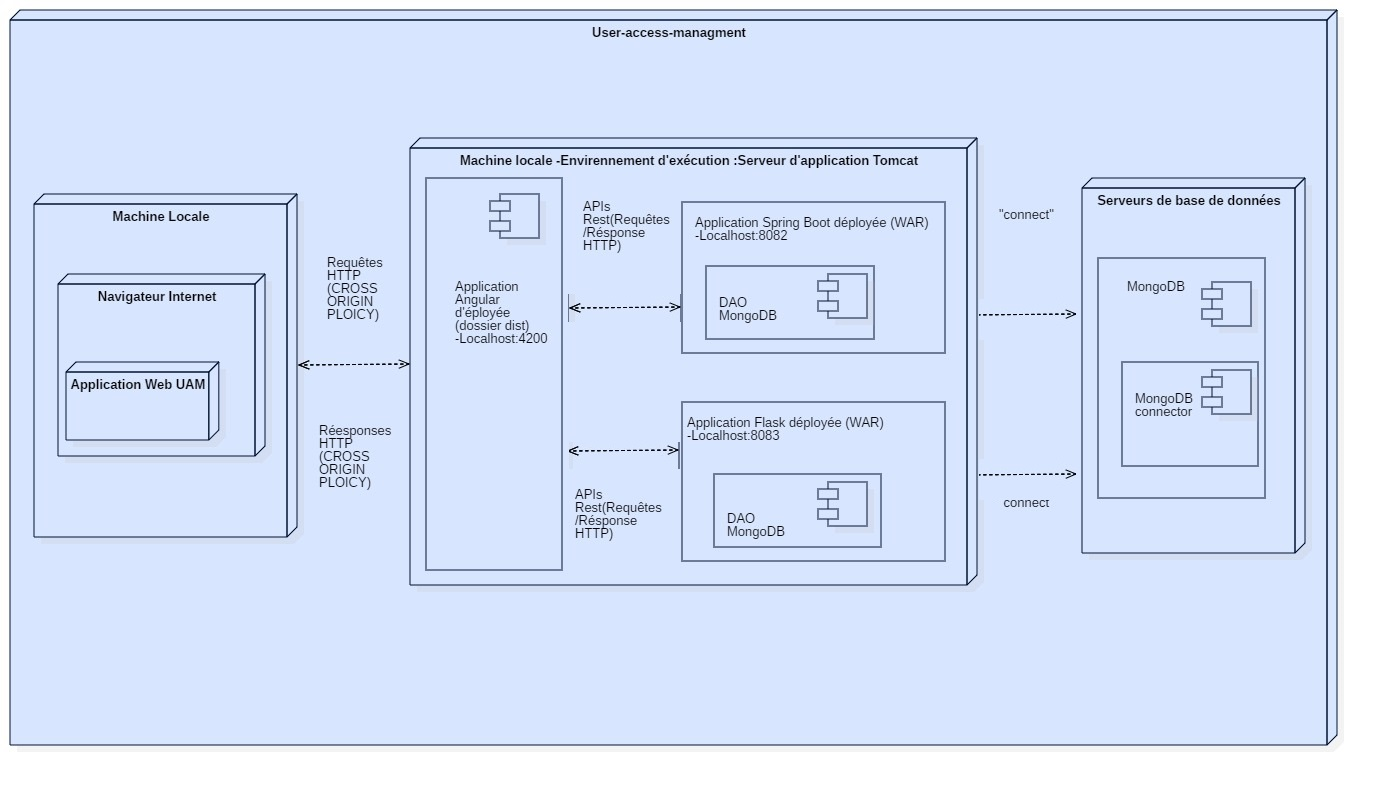
\includegraphics[width=1\columnwidth]{chapitres/chapitre8/figures/DeploymentDiagram1.jpg}}
\caption{Diagramme de déploiement : architecture physique}
\label{fig:DeploymentDiagram1}
\end{figure}

\section{Environnement de travail}
\subsection{Environnement logiciel}
\subsubsection*{Apache Tomcat 9}
Tomcat est un serveur d'applications Java. Nous avons déjà présenté ce qu'est une application web. Elle permet de générer une réponse HTML à une requête après avoir effectué un certain nombre d'opérations (connexion à une base de données, à un annuaire LDAP...). Pour le client (un navigateur web en général), il n'y a pas de différence avec une page web statique : il reçoit toujours du HTML, seul langage qu'il comprend. Seule la manière dont la réponse est formée côté serveur change.
\begin{figure}[!ht]\centering

\includegraphics[width=0.4\textwidth]{chapitres/chapitre8/figures/apachtomcat.png}
\caption{Apache Tomcat logo}
\label{fig:apachtomcat}
\end{figure}
\section{Accès à l'application monitoring des transactions }	
L'accès au l'application monitoring des transactions sera matérialisé par un lien web sur l'onglet "Identification du client". Il sera accessible en vue normale si le CA souhaite regarder les dernières transactions de son client et en vue KYC.

Depuis CBS, il conviendra de matérialiser l’accès à ce dashboard par un mécanisme similaire.

Lors de la revue KYC, le chargé d'affaires devra impérativement avoir revu les transactions pour pouvoir valider le KYC. Dans le cas où la revue n'a pas été effectuée, un message s'affichera : 

"Avant de valider l'authentification de l'acteur, vous devez vérifier le profil de transactions de de ses clients, accessible via le lien "l'application monitoring des transactions".
\newline
La figure suivante présente une interface de CRM modifier à cause de confidentialités et cette interface présente le scénario de l'accès à notre application
\newpage
\begin{figure}[!ht]\centering
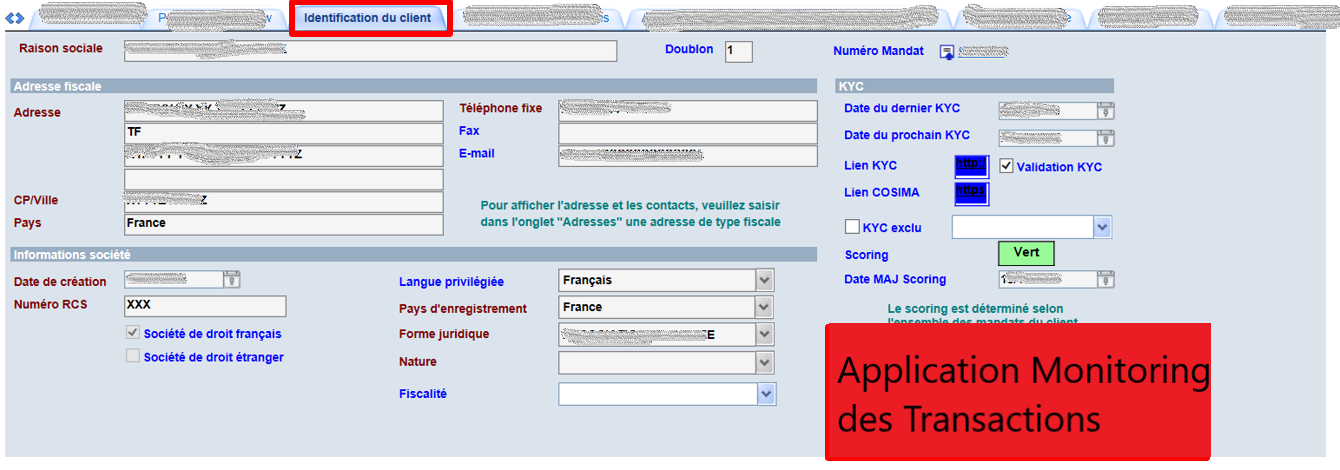
\includegraphics[width=1\textwidth]{chapitres/chapitre8/figures/acces.png}
\caption{Accès à l'application monitoring des transactions}
\label{fig:acces}
\end{figure}
\section*{Conclusion}
Au cours de ce chapitre nous avons présenté et argument\'e notre architecture et la structure générale pour mise en place notre application.
\include{chapitres/chapitre9}
\include{chapitres/chapitre10}
\include{chapitres/chapitre11}
% \include{chapitres/chapitre12}
\fancyhead[R]{\ungaramond\small\textbf{}}
\phantomsection\addcontentsline{toc}{chapter}{General Conclusion}\textcolor{white}{I} %\textcolor{white}{I} inclure\textcolor{white}{I} dans\textcolor{white}{I} TdM

\begin{center}
\ungaramond{\textbf{\LARGE{General Conclusion}}}

\end{center}
In conclusion, our project has demonstrated the potential of Agile DevOps in cloud computing and DevOps. By implementing a comprehensive PaaS environment, we have shown how businesses can leverage the power of cloud technology to streamline the application development and delivery process. 

Our project's focus on networking services, authentication and authorization services, distributed storage, CICD tools, and DevOps pipelines enables businesses to deploy applications rapidly and reliably. 

Our networking services, including layer 7 and 4 load balancers, and a TLS certificate provisioner, ensure that the application can be accessed securely and efficiently. 

Our authentication and authorization service provides secure access to the ecosystem, while our distributed storage backend ensures that data is stored reliably and efficiently. 

Our CICD tools and DevOps pipelines enable businesses to automate and streamline the application development and delivery process, reducing the time to market. 

Furthermore, we have implemented a resilient disaster recovery strategy to ensure business continuity in case of any disruptions. 

The success of our project serves as a testament to the importance of Agile DevOps in modern-day software development and delivery. Our project's implementation the PaaS environment can be used as a blueprint for businesses looking to implement a comprehensive PaaS environment in the cloud. 

Overall, our project has shown that by leveraging Agile DevOps in cloud computing, businesses can rapidly and reliably deploy applications, enabling them to stay ahead of the competition. 

\bibliographystyle{unsrt}
\nocite{*}
\bibliography{bibliographie}



%


%----------------------------------------------------------------------------------------
%	TITLE PAGE
%----------------------------------------------------------------------------------------
\fancyhead[R]{\ungaramond\small\textbf{ }}
\thispagestyle{empty}
 \begin{tikzpicture}[remember picture,overlay]
   \node at (current page.center) {
\includegraphics[width=\pdfpagewidth,height=\pdfpageheight]{frontmatter/remerciements/garde1.png}};
 \end{tikzpicture}
\clearpage
\clearpage\thispagestyle{empty}\addtocounter{page}{-5}


%----------------------------------------------------------------------------------------

\end{document}
